% =====================================================================
% GPU-resident generalist study. Tables tab_gen_*.tex, figures study_*.pdf and the numbers \gv{...} are generated by site/build_data.py
% from outputs/study/warp_ppo/*; do not edit the numbers by hand. Simulation only.
% =====================================================================
\section{GPU-Resident Training: Setup}\label{sec:gpu}
The study so far used one simulator process per run. To train one policy across terrains, floor materials and robot designs we moved the whole learning loop onto the GPU and then asked, in order, what limits such a policy and what structure removes the limit.

\subsection{Engines and validation}\label{sec:engines}
The reference engine is MuJoCo (CPU, float64, implicit-fast integrator, with the contact-frame correction of \S\ref{sec:system}). The training engine is MuJoCo-Warp 3.17 (GPU, float32) with the same correction as a custom kernel inside a CUDA graph. Before any policy was trained on it, an LQR on 17 designs gave the same fall or no-fall outcome in 94.6\,\% of speed tests (193 of 204) and 96.1\,\% of push tests (784 of 816), with speed ratios of non-falling runs within 0.01; one CPU process reaches 1.36k control steps/s and Warp 355k at 4096 worlds, a factor of about 260 (engine report \texttt{experiments/mjx\_port/REPORT.md}). Warp is not bit-reproducible and individual trajectories spread more than on the CPU. Observation, reward, resets, command sampling, pushes and PPO all run on the GPU through torch views of the Warp arrays; removing host synchronisations (29 to 1 per control step) raised an end-to-end 12M-step run from 52k to 67k environment steps/s with the same learning curve. Policy-transfer checks between the engines were made before the correction described below and are not reported. One quirk of the original environment is kept on purpose: its \texttt{motor\_state} input reads \texttt{qvel[joint.id]}, which indexes the base free joint, so the policies receive scaled base-velocity components in those three slots and never the wheel rates; a first GPU port that read the true wheel rates failed on the CPU engine until the quirk was copied.

\paragraph{Engine pitfall: stale subtree mass.} In a batched MuJoCo-Warp model with per-world masses the derived \texttt{body\_subtreemass} must be recomputed too: the engine locates each subtree's centre of mass by dividing mass-weighted positions by it and uses that point as the dynamics reference, so a stale value shifts the reference by a fraction of the distance from the world origin (our tiles lie up to 12\,m away) and the error vanishes at the nominal mass. Our code randomised the base and ball masses but not \texttt{body\_subtreemass}, so every run and evaluation with randomisation on was affected until the fix; randomisation off was not. Evidence (LQR alone, clean flat world, 64 worlds, falls at 0.3/0.6\,m/s): nominal 0.12/0.16; ball-mass randomisation 0.41/0.81 before and 0.17/0.23 after the fix; a ball mass fixed at 0.63 to 2.0 times nominal gave 0.62 to 1.00 before. Planar-model checks and changes of the integral gain, control cost and ball inertia did not remove it, whereas recomputing the constants for one changed mass did. The fix recomputes the subtree masses from the per-world masses at every reset. All randomised results in this paper come from runs made after the fix.



\subsection{The model-based controller in discrete time}\label{sec:dlqr}
A continuous LQR with light rotors has a pole near $-135\,\mathrm{s}^{-1}$ at 100\,Hz and is unstable when sampled, so the controllers used with the GPU stack are designed in discrete time at the control period $T=0.01$\,s. With $(A_d,B_d)$ the zero-order-hold discretisation of $(A,B_s)$ and the same weights ($Q T$, $R T$), the discrete Riccati solution gives $K_d=(R T+B_d^{\top}XB_d)^{-1}B_d^{\top}XA_d$. For the nominal robot $K_d=(-0.001,\ \gv{model.Kd1},\ \gv{model.Kd2},\ \gv{model.Kd3})$ and the continuous gain is $K=(-0.001,\ \gv{model.Kc1},\ \gv{model.Kc2},\ \gv{model.Kc3})$ with $\tau=-K(s-s_{\mathrm{ref}})$ (the entries are negative because $B_s$ has a positive torque convention on $\varphi$ and a negative one on $\theta$; \S\ref{sec:lqr} quotes the magnitudes). The reference governor, the slow integral on the measured velocity and the yaw loop are as in \S\ref{sec:lqr}; a batched version runs on the GPU with one gain per design.

\subsection{Learning problem as coded}\label{sec:gpurl}
\textbf{Observation.} The policy sees 25 numbers: orientation rotation vector (3), body angular velocity (3) and linear velocity (3), the \texttt{motor\_state} slots described above (3), the previous action (3), the command $(v_x,v_y,\omega_z)$ (3), sine and cosine of the body yaw (2), the velocity-error integral $\xi_v\leftarrow\mathrm{clip}(\xi_v+(c-v)\,0.01,\pm1)$ (2) and the goal error divided by 2 and clipped (2) with a goal flag (1). Optional extras are a stack of the last $K=8$ pairs of policy-visible observation and action, a 6-number design vector and a sensor vector. Gaussian noise ($\sigma=0.01$; $0.25\sigma$, $2\sigma$, $\sigma$ on orientation, angular and linear velocity) is added to the first nine slots when randomisation is on. With history 8 and the design vector the main runs see 255 numbers. The action is $a\in[-1,1]^3$ with wheel torque $\mathrm{clip}(\kappa\tau_d a,\pm\tau_d)$, $\tau_d$ the design's torque limit and $\kappa\sim\mathcal U(0.85,1.15)$.

\textbf{Commands and goals.} Velocity commands are resampled every 300 control steps: zero with probability 0.1, otherwise speed $\mathcal U(0,1.2)\sqrt{r_{\mathrm{ball}}/0.09}$\,m/s, direction $\mathcal U(0,2\pi)$, yaw rate $\mathcal U(-1,1)$\,rad/s; episodes last 800 steps. In goal mode the command is the saturating proportional rule
\begin{equation}
c_{xy}=\min\big(k_g\lVert g-p\rVert,\ v_{\max}f\big)\frac{g-p}{\lVert g-p\rVert},\quad k_g=1.5\,\mathrm{s}^{-1},\quad c_{xy}=0\ \text{if}\ \lVert g-p\rVert<0.05\,\mathrm{m},\quad c_\omega=0,
\end{equation}
so speed is free up to a cap while the tracking reward still applies. Goals are drawn 0.7 to 1.8\,m away (within 1.3\,m of the tile centre); a world with waypoints left draws the next goal on arrival within 0.2\,m. With \emph{cross-focus} a goal is, with probability 0.6, placed 1.1 to 1.3\,m from the tile centre along a tile axis, so reaching it means crossing the terrain feature.

\textbf{Reward.} With $e=\lVert v-c_{xy}\rVert$, $\hat c=c_{xy}/\lVert c_{xy}\rVert$, $p=v\cdot\hat c$, $e_\omega=|\omega_z-c_\omega|$, $\ell=\Delta_{xy}\!\cdot\hat c/\Delta_z$ the lean along the command ($\Delta$ the body position minus the ball centre) and $\beta=\operatorname{atan2}(\lVert\Delta_{xy}\rVert,\Delta_z)$ the ball offset, the reward of \texttt{train\_dev.py} is
\begin{align}
\mathrm{raw}&=(\lVert c\rVert-e)+\tfrac12e^{-e^2/0.25^2}+\tfrac12(|c_\omega|-e_\omega)+\tfrac14e^{-e_\omega^2/0.5^2}+\tfrac12\,\mathbb 1[\lVert c\rVert>0.05]\Big(1-\mathrm{clip}\big(\tfrac{p}{\lVert c\rVert},0,1\big)\Big)\mathrm{clip}\big(\tfrac{\ell}{0.3},-1,1\big),\\
r_t&=2.5\,w_{\mathrm{trk}}\,\mathrm{raw}-w_{\mathrm{pen}}\Big[5{\times}10^{-4}\lVert a_t\rVert^2+0.1\lVert a_t-a_{t-1}\rVert^2+0.25\big(\tfrac{\beta}{30^\circ}\big)^2\Big]+\begin{cases}0.1&\text{upright}\\-2&\text{fall.}\end{cases}
\end{align}
The weight $w_{\mathrm{trk}}$ multiplies the whole bracket (1, 2 or 4 in our runs) and $w_{\mathrm{pen}}$ the three penalties. A fall is a tilt above $70^\circ$, $\beta>30^\circ$ or a non-finite state; leaving the 2.9\,m tile square truncates the episode without penalty, and time-limit truncations bootstrap the value.

\textbf{PPO.} A diagonal Gaussian policy with a state-independent log standard deviation (initial $-1$) and a tanh MLP (three hidden layers of 512 units in the main runs). The loss is the clipped surrogate plus a value term and \emph{no entropy bonus}:
\begin{equation}
\mathcal L=-\mathbb E\big[\min(\rho_t\hat A_t,\ \mathrm{clip}(\rho_t,0.8,1.2)\hat A_t)\big]+0.25\,\mathbb E\big[(V_\phi-\hat R_t)^2\big],\quad \hat A_t=\sum_{l\ge0}(\gamma\lambda)^l\delta_{t+l},
\end{equation}
with $\gamma=0.995$, $\lambda=0.95$, 4096 worlds $\times$ 64 steps per iteration, 5 epochs of 8 minibatches, Adam with learning rate $3{\times}10^{-4}\to3{\times}10^{-5}$ and gradient-norm clip 0.5, advantage normalisation per minibatch and an early stop at approximate KL 0.03. Rewards are divided by the running standard deviation of the discounted return and clipped at 10; observations are normalised by running statistics. The actor sees only deployable inputs; the \emph{asymmetric critic} also sees floor friction and softness, base and ball mass offsets, torque scale, wheel damping, a 34-number height scan and the design vector.

\subsection{LQR plus a bounded learned residual}\label{sec:resgpu}
The environment applies $a=\mathrm{clip}(a_{\mathrm{LQR}}+r_s\,a_\pi,\pm1)$ with $a_\pi$ the policy output and $r_s$ the \emph{residual authority}; the LQR runs inside the environment at every control step from the simulator state with one gain set per design, and latency, torque scaling and pushes act on the sum. The output layer starts near zero so training starts from the plain LQR. Fig.~\ref{fig:arch} sketches the architecture. An interleaved gate $a=(1-g)a_{\mathrm{LQR}}+g\,a_\pi$ was tried on the CPU engine and collapsed to the pure LQR.
\begin{figure}[t]\centering
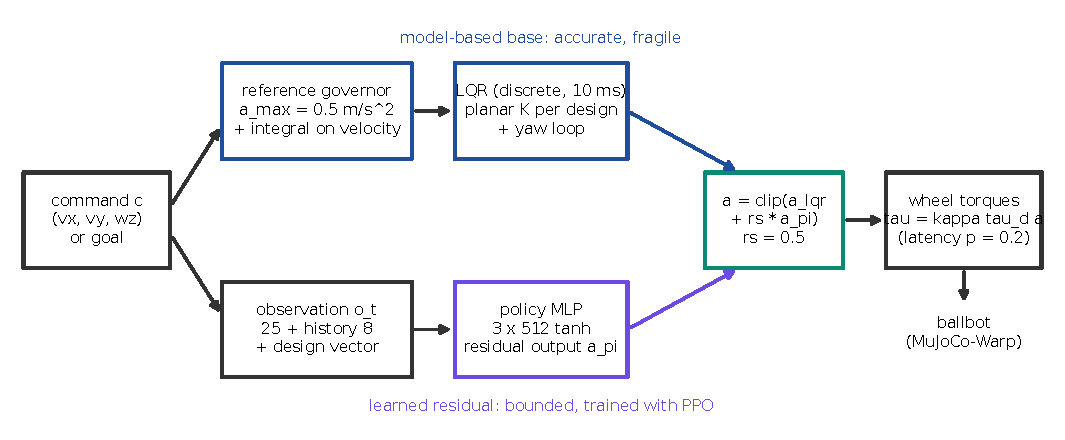
\includegraphics[width=\columnwidth]{figures/study_arch.pdf}
\caption{Architecture of the LQR plus residual controller (schematic, no data). Blue: model-based path using the simulator state; violet: learned path using the noisy observation; teal: the sum with authority $r_s$. Engine: Warp GPU. Randomisation and noise act as in Table~\ref{tab:gen_dr}.}\label{fig:arch}
\end{figure}

\subsection{Terrain, floors, designs and randomisation}\label{sec:world}
MuJoCo-Warp shares one height field across worlds, so terrain variety is a 24\,m map of $8\times8$ tiles of 3\,m (3.4\,cm cells, $h=B+g(x)+g(y)$ with features at least 0.5\,m from the tile centre so that any heading meets them; Fig.~\ref{fig:tiles}, Table~\ref{tab:gen_tiles}). A world picks a tile and a start within $\pm0.3$\,m of its centre; severity is drawn once per tile and the map is generated with a fixed seed, so training and evaluation share the same 64 tiles. Seven floor classes (Table~\ref{tab:gen_surfaces}) set the ball-floor friction and contact time constant (plausible, not measured). Thirteen designs share one topology and their differing model fields are batched per world (Table~\ref{tab:gen_designs}); eleven form the training set, after a per-design fall breakdown showed that two (half scale and very light rotors) were effectively unlearnable. Table~\ref{tab:gen_dr} lists the randomisation.
\begin{figure}[t]\centering
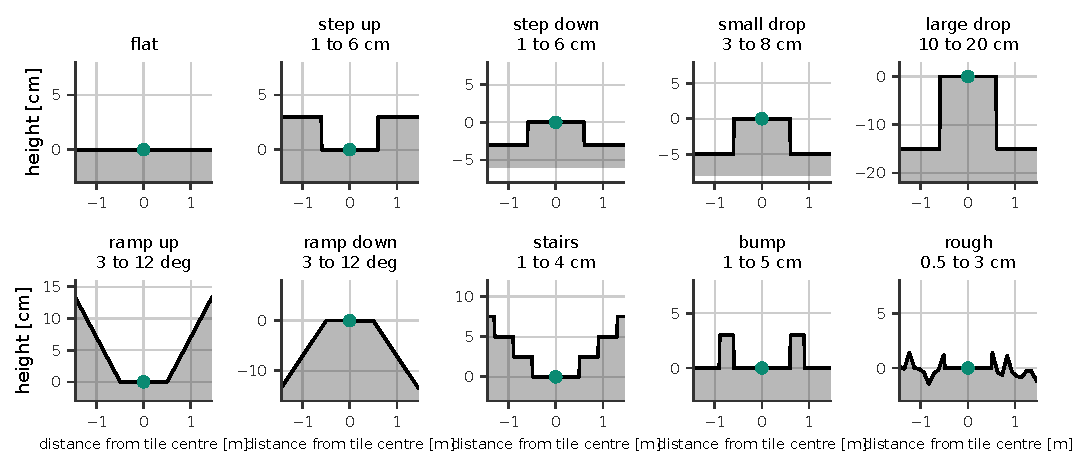
\includegraphics[width=\columnwidth]{figures/study_tiles.pdf}
\caption{Terrain tile library: cross-section through the tile centre (dot) at a representative severity; titles give the training range. Geometry only: no engine, randomisation, noise, worlds or seeds apply (map seed 0).}\label{fig:tiles}
\end{figure}
\begin{table}[t]\centering\footnotesize
\caption{Terrain tile library (geometry only; map 24\,m, 3\,m tiles, truncation outside a 2.9\,m square).}\label{tab:gen_tiles}
\resizebox{\columnwidth}{!}{%
\begin{tabular}{llp{4.2cm}c}\toprule
Terrain kind & Severity range & Profile & Tiles of 64\\\midrule
flat & none & no feature & 7\\
step up & 1 to 6 cm & single raised step 0.6 m from the centre on each axis & 7\\
step down & 1 to 6 cm & robot stands on a plateau, floor drops by the severity & 7\\
small drop & 3 to 8 cm & drop of 3 to 8 cm & 7\\
large drop & 10 to 20 cm & drop of 10 to 20 cm & 6\\
ramp up & 3 to 12 deg & slope over 1.0 m starting 0.5 m from the centre & 6\\
ramp down & 3 to 12 deg & descending slope over 1.0 m & 6\\
stairs & 1 to 4 cm & 2 to 3 treads of 0.4 m, riser = severity & 6\\
bump & 1 to 5 cm & slab 0.3 m wide, 0.6 m from the centre & 6\\
rough & 0.5 to 3 cm & smooth two-octave noise outside a flat 0.5 m start zone & 6\\
\bottomrule\end{tabular}}
\end{table}

\begin{table}[t]\centering\footnotesize
\caption{Floor material classes (plausible, not measured).}\label{tab:gen_surfaces}
\resizebox{\columnwidth}{!}{%
\begin{tabular}{lcc}\toprule
Floor class & Friction $\mu$ & Contact time constant [s]\\\midrule
concrete & 0.9 & 0.020\\
hardwood & 0.6 & 0.020\\
carpet & 1.1 & 0.045\\
grass & 0.8 & 0.050\\
gravel & 0.7 & 0.030\\
wet tile & 0.3 & 0.020\\
rubber & 1.3 & 0.020\\
\bottomrule\end{tabular}}
\end{table}

\begin{table*}[t]\centering\footnotesize
\caption{The 13 compiled designs (eleven used in training).}\label{tab:gen_designs}
\resizebox{\textwidth}{!}{%
\begin{tabular}{llccccccc}\toprule
Design & What it changes & Body mass [kg] & Ball mass [kg] & COM height l [m] & Rotor inertia [kg m$^2$] & Torque limit [N m] & Contact zenith [deg] & In training set\\\midrule
nom & reference robot & 3.85 & 0.168 & 0.131 & 0.005 & 30 & 51 & yes\\
zhigh & ballast raised: COM height about 1.9 times nominal & 3.85 & 0.168 & 0.254 & 0.005 & 30 & 51 & yes\\
zlow & ballast lowered: COM height about 0.67 times nominal & 3.85 & 0.168 & 0.087 & 0.005 & 30 & 51 & yes\\
kb4 & ball mass x4 & 3.85 & 0.672 & 0.131 & 0.005 & 30 & 51 & yes\\
bal4 & body ballast x4 (body mass 3.5 times nominal, pushes scaled) & 13.45 & 0.168 & 0.124 & 0.005 & 30 & 51 & yes\\
J02 & wheel rotor inertia x4 & 3.85 & 0.168 & 0.131 & 0.02 & 30 & 51 & yes\\
tau6 & torque limit 6 N m (one fifth) & 3.85 & 0.168 & 0.131 & 0.005 & 6 & 51 & yes\\
bal025 & ballast x0.25 (body mass 0.38 times nominal) & 1.45 & 0.168 & 0.145 & 0.005 & 30 & 51 & yes\\
kb025 & ball mass x0.25 & 3.85 & 0.042 & 0.131 & 0.005 & 30 & 51 & yes\\
zeta41 & wheel contact zenith 41 deg (nominal 51) & 3.85 & 0.168 & 0.132 & 0.005 & 30 & 41 & yes\\
zeta66 & wheel contact zenith 66 deg & 3.85 & 0.168 & 0.129 & 0.005 & 30 & 66 & yes\\
s0.5 & half scale (all lengths x0.5, masses x0.125) & 0.48 & 0.021 & 0.065 & 0.0001563 & 1.875 & 51 & no (dropped)\\
J0005 & rotor inertia x0.1 & 3.85 & 0.168 & 0.131 & 0.0005 & 30 & 51 & no (dropped)\\
\bottomrule\end{tabular}}
\end{table*}

\begin{table*}[t]\centering\footnotesize
\caption{Domain randomisation ranges (configs/env/dz\_nom.yaml and train\_dev.py).}\label{tab:gen_dr}
\resizebox{\textwidth}{!}{%
\begin{tabular}{p{2.6cm}p{6cm}p{2.4cm}p{3.6cm}}\toprule
Quantity & Range & When & Notes\\\midrule
Robot design & one of 11 designs, uniform & per episode & Table C\\
Base mass and ball mass & each times (1 plus uniform plus or minus 0.15) & per episode & independent draws\\
Wheel-ball transverse friction & times (1 plus uniform plus or minus 0.20) & per episode & the cross-roller direction of the anisotropic pair\\
Wheel damping & uniform 0.07 to 0.15 N m s times the design's nominal damping over 0.1 & per episode, each wheel & master scale widens the spread around 0.1\\
Torque scale & 1 plus uniform plus or minus 0.15 & per episode & applied to the commanded torque\\
Action latency & with probability 0.2 the previous action is applied instead & per control step & probability capped at 0.6 when scaled\\
Observation noise & Gaussian, sigma 0.01 (orientation 0.25 sigma, angular velocity 2 sigma, linear velocity 1 sigma) & per control step & slots 0 to 8 only\\
Pushes & horizontal force 5 to 20 N (times the design push factor), random direction, 5 control steps (50 ms) & every 2 to 4 s & factor = push range of the design over 20 N\\
Pulls & horizontal force 3 to 12 N, random direction, 0.5 to 2 s & every 4 to 10 s & only in runs with pulls on; not scaled per design\\
Floor material & one of 7 classes; friction times (1 plus uniform plus or minus 0.15) & per episode & Table B\\
Terrain tile and start & uniform over 64 tiles; start offset uniform plus or minus 0.3 m; start yaw uniform over a full turn & per episode & Table A\\
Master scale (wide runs) & multiplies mass, friction, torque, damping spread, latency probability and noise ranges; 1 to 1.75 over the first half of training & per iteration & does not scale pushes or pulls\\
\bottomrule\end{tabular}}
\end{table*}


\subsection{Evaluation protocols and metrics}\label{sec:gpueval}
All GPU evaluations use a deterministic policy (the Gaussian mean), a fixed seed and no command resampling; the first fall of a world freezes it. (i)~\emph{Clean flat benchmark}: a perfectly flat 24\,m world (interior tiles only, at least 7.5\,m from the border: the first version used border tiles, and with tile exits disabled a robot driving outward left the height field and was counted as a fall; a per-fall position record showed that most recorded flat falls were such drop-offs, the benchmark was fixed and the flat rows of every battery were re-run; the error and achieved-speed metrics, computed over surviving worlds, are unaffected by the artefact), nominal design, randomisation (hence noise, latency and pushes) off, a constant command of 0.3, 0.6 or 0.9\,m/s at a random heading, 800 steps; 64 worlds per row (two nominal-design copies of 32 random start poses and headings; 32 for the LQR calibration). Steady-state error $\lVert v-c\rVert$ and achieved/commanded speed $v\cdot c/\lVert c\rVert^2$ are averaged over steps 300 to 799 of worlds still upright; the fall rate is the share of worlds that fell at any time. (ii)~\emph{Velocity task on the tiles}: 0.3\,m/s at a random heading, 11 designs $\times$ 10 terrain kinds $\times$ 16 repeats (1760 worlds), randomisation and floor classes on; \emph{undisturbed} means pushes and pulls off, \emph{disturbed} means pushes of 5 to 20\,N (scaled per design) and pulls of 3 to 12\,N at full strength. (iii)~\emph{Goal task}: a goal 1.1\,m away at a random heading, the same layout; success is reaching within 0.2\,m before any fall, with the median time over successful worlds and success per terrain kind (176 worlds). (iv)~\emph{Disturbance scaling}: pushes and pulls multiplied together by 0 to 1. With 1760 worlds a fall rate near 0.5 has a binomial standard error of about 0.012, a terrain kind about 0.04 and a 64-world row about 0.06; the seed-to-seed spread of a recipe is about 0.03 to 0.06 (Fig.~\ref{fig:seeds}). Every table and figure states engine, randomisation, noise, worlds per cell, seeds and protocol.

% =====================================================================
\section{GPU Generalist: Results}\label{sec:gpuresults}
All randomised results in this section come from runs trained and evaluated on the corrected engine (\S\ref{sec:engines}); earlier randomised results are superseded and omitted. Evaluations with randomisation off were never affected. Recipes (all 11 designs, 200M steps unless stated): pure learning (no LQR, 300M steps); LQR + residual with authority 0.5 at the standard randomisation ranges (A, two seeds); the same with ranges ramped to 1.75 times over the first half of training (B, two seeds); a soft LQR base (control cost $\times3$, reference acceleration 0.3\,m/s$^2$) with the 1.75 ramp (C, two seeds) and with authority 0.75 (one seed).

\subsection{Baselines on the CPU engine}
\begin{table*}[t]\centering\footnotesize
\caption{Baseline controllers on the CPU engine (selected rows of Table~\ref{tab:tracking}). Engine: CPU (MuJoCo 3.13, float64, implicit-fast, contact-frame fix). Domain randomisation: off (nominal robot). Observation noise: off. Worlds per cell: 1 robot per condition, 2 repeats per speed and direction (8 directions); 30 random-command episodes. Seeds: 1 per row unless two are listed. Protocol: scripts/study/eval\_control.py and eval\_falls.py, deterministic policies. The 1.0 m/s ratio of the LQR averages trials that mostly fall; the LQR falls in every 1 m/s trial of the study log.}\label{tab:gen_cpu}
\resizebox{\textwidth}{!}{%
\begin{tabular}{lccccc}\toprule
Controller & Achieved/commanded at 0.5 m/s & at 1.0 m/s & Velocity RMSE, commands up to 1 m/s [m/s] & Heading-test error [m/s] & Falls in 30 random-command episodes\\\midrule
LQR on the derived model (lqr) & 1.04 & 1.06 & 0.05 & 0.02 & 18/30\\
PPO, spin cap 1 rad/s, from scratch (trk\_f\_s0) & 0.98 & 0.91 & 0.12 & n/a & 16/30\\
same, seed 1 (trk\_f\_s1) & 1.09 & 0.95 & 0.11 & n/a & 14/30\\
trk\_f continued, smoother (trk\_g\_s0) & 0.99 & 0.87 & 0.12 & n/a & 11/30\\
PPO fine-tuned under DR, pushes 10 to 35 N (rob\_b\_s0) & 0.28 & 0.27 & 0.52 & 0.37 & 8/30\\
PPO from scratch under DR (narrow damping) (robs\_b\_s0) & 0.50 & 0.51 & 0.37 & 0.27 & 3/30\\
robs\_b + outer velocity integral (robs\_b\_ki1) & 1.01 & 0.79 & 0.19 & 0.06 & 8/30\\
LQR + residual (beta 0.1, zero-init) (res\_c\_s0) & 1.03 & 1.05 & 0.08 & 0.02 & 3/30\\
res\_c continued, beta 0.2, DR + pushes (res\_d\_s0) & 1.33 & 0.75 & 0.32 & 0.13 & 15/30\\
\bottomrule\end{tabular}}
\end{table*}

Table~\ref{tab:gen_cpu} repeats the CPU results that carried forward (the full list is Table~\ref{tab:tracking}): the LQR is accurate and fragile, the randomised-from-scratch PPO policy is robust and timid, and a small-authority residual on the LQR keeps the LQR's precision.

\subsection{Tracking accuracy and the LQR calibration (clean flat world)}
On the clean flat benchmark (Table~\ref{tab:gen_flat}, Fig.~\ref{fig:tracking}) the pure-learning policy reaches \gv{flat.g12_pure_s0.0.3.ratio}, \gv{flat.g12_pure_s0.0.6.ratio} and \gv{flat.g12_pure_s0.0.9.ratio} of the commanded speed at 0.3, 0.6 and 0.9\,m/s (error \gvt{flat.g12_pure_s0.0.3.err} to \gvt{flat.g12_pure_s0.0.9.err}\,m/s). The batched GPU LQR on the same worlds (re-measured on interior tiles after the map-edge correction, 64 worlds; S92 addendum) tracks exactly up to 0.6\,m/s (error \gvt{lqr.err03} and \gvt{lqr.err06}\,m/s, ratio 1.00, no falls), \gv{cmp.lqr_acc_min} to \gv{cmp.lqr_acc_max} times more accurate than pure learning, so the shortfall is a policy deficiency and not a limit of the robot; at 0.9\,m/s the LQR alone falls in \gv{lqr.fall09} of worlds, its speed wall near 1\,m/s, which the learned residual removes (the residual controllers fall 0.00 to 0.02 there at the same accuracy). The residual keeps the LQR's accuracy (error \gvt{flat.g12_res_s0.0.3.err} to \gvt{flat.g12_res_s0.0.9.err}\,m/s on seed 0 and \gvt{flat.g12_res_s1.0.3.err} to \gvt{flat.g12_res_s1.0.9.err} on seed 1; \gvp{cmp.relerr_min} to \gvp{cmp.relerr_max}\,\% of the command) with fewer falls at 0.9\,m/s; the flat 0.9\,m/s fall rate differs between seeds (\gv{flat.g12_res_s0.0.9.fall} and \gv{flat.g12_res_s1.0.9.fall}; 64 worlds, standard error about 0.05).
The fall column of Table~\ref{tab:gen_flat} is the re-run on interior tiles after the map-edge correction (\S\ref{sec:gpueval}); the recommended controller does not fall at any speed in it. The LQR-alone row is the interior-tile re-measurement of the same addendum.
\begin{table*}[t]\centering\footnotesize
\caption{Clean flat-world velocity-tracking benchmark, corrected engine. Cells: steady-state error [m/s] / achieved over commanded speed / fall rate. Engine: Warp GPU (MuJoCo-Warp 3.17, float32), corrected for the S69 stale-subtree-mass error. Domain randomisation: off. Observation noise: off. Worlds per cell: 64 per cell. Seeds: one per row as listed (seeds 0 and 1 where both are shown). Protocol: perfectly flat 24 m world on interior tiles (at least 7.5 m from the map border, the S92 correction), nominal design, constant velocity command at a random heading, 800 control steps, error and achieved/commanded speed averaged over steps 300 to 799 of worlds still upright, falls = share of worlds that fell (eval\_battery.py; every flat row re-run after S92). Error is the Euclidean velocity error in m/s. All learned rows are corrected-engine runs. The LQR-alone row is the interior-tile re-measurement of the S92 addendum (source: lqr\_flat\_interior.log); a dagger marks values taken from the log.}\label{tab:gen_flat}
\resizebox{\textwidth}{!}{%
\begin{tabular}{lcccc}\toprule
Controller & 0.3 m/s: err / achieved / falls & 0.6 m/s & 0.9 m/s & Seed\\\midrule
LQR alone & 0.014 / 1.00 / 0.00 & 0.017 / 1.00 / 0.00 & 0.026 / 1.00 / 0.91 & n/a (no learning)\\
pure learning (no LQR), 300M steps (seed 0) & 0.130 / 0.60 / 0.00 & 0.260 / 0.58 / 0.00 & 0.406 / 0.55 / 0.00 & seed 0\\
LQR + residual 0.5, standard randomisation (seed 0) & 0.031 / 0.93 / 0.00 & 0.056 / 0.94 / 0.00 & 0.064 / 0.98 / 0.02 & seed 0\\
LQR + residual 0.5, standard randomisation (seed 1) & 0.025 / 0.95 / 0.00 & 0.038 / 0.97 / 0.00 & 0.048 / 0.99 / 0.00 & seed 1\\
LQR + residual 0.5, randomisation ramped to 1.75x (seed 0) & 0.027 / 0.95 / 0.00 & 0.046 / 0.97 / 0.00 & 0.057 / 0.99 / 0.02 & seed 0\\
LQR + residual 0.5, randomisation ramped to 1.75x (seed 1) & 0.013 / 1.00 / 0.00 & 0.021 / 1.00 / 0.00 & 0.041 / 1.02 / 0.00 & seed 1\\
soft LQR base (R x3, a\_max 0.3), ramped to 1.75x (seed 0) & 0.032 / 0.91 / 0.00 & 0.068 / 0.93 / 0.00 & 0.098 / 0.95 / 0.00 & seed 0\\
soft LQR base (R x3, a\_max 0.3), ramped to 1.75x (seed 1) & 0.039 / 0.90 / 0.00 & 0.084 / 0.92 / 0.00 & 0.123 / 0.94 / 0.00 & seed 1\\
soft LQR base, authority 0.75 (seed 0) & 0.050 / 0.86 / 0.00 & 0.136 / 0.81 / 0.00 & 0.188 / 0.84 / 0.02 & seed 0\\
ramped 1.75x, fall penalty 5 (was 2) (seed 0) & 0.027 / 0.95 / 0.00 & 0.044 / 0.98 / 0.02 & 0.062 / 1.01 / 0.00 & seed 0\\
soft base, fall penalty 5 (seed 0) & 0.025 / 0.95 / 0.00 & 0.053 / 0.96 / 0.00 & 0.102 / 0.96 / 0.02 & seed 0\\
ramped 1.75x, push and pull strength ramped 0.2 to 1 (seed 0) & 0.026 / 0.96 / 0.00 & 0.045 / 0.97 / 0.00 & 0.061 / 1.00 / 0.02 & seed 0\\
ramped 1.75x + edge starts + depth sensor (seed 0) & 0.014 / 1.00 / 0.00 & 0.027 / 0.99 / 0.00 & 0.044 / 1.00 / 0.02 & seed 0\\
ramped 1.75x + edge starts, blind control (seed 0) & 0.019 / 0.99 / 0.02 & 0.033 / 0.99 / 0.00 & 0.046 / 1.00 / 0.00 & seed 0\\
pure learning (no LQR), 300M steps (seed 1) & 0.103 / 0.67 / 0.11 & 0.246 / 0.59 / 0.00 & 0.421 / 0.54 / 0.00 & seed 1\\
ramped 1.75x, trained with the ball retainer (arrestors at 100 deg) (seed 0) & 0.049 / 0.86 / 0.00 & 0.140 / 0.81 / 0.00 & 0.188 / 0.86 / 0.00 & seed 0\\
ramped 1.75x, trained with the ball retainer (arrestors at 100 deg) (seed 1) & 0.048 / 0.87 / 0.00 & 0.096 / 0.87 / 0.00 & 0.115 / 0.91 / 0.00 & seed 1\\
pure learning, trained with the retainer (seed 0) & 0.087 / 0.73 / 0.00 & 0.196 / 0.69 / 0.00 & 0.335 / 0.64 / 0.00 & seed 0\\
pure learning, trained with the retainer (seed 1) & 0.060 / 0.82 / 0.02 & 0.172 / 0.72 / 0.00 & 0.325 / 0.65 / 0.02 & seed 1\\
retainer, authority 0.5, tracking weight x3 (seed 0) & 0.039 / 0.88 / 0.00 & 0.177 / 0.74 / 0.00 & 0.201 / 0.84 / 0.00 & seed 0\\
retainer, authority 0.15 (seed 0) & 0.016 / 0.99 / 0.00 & 0.023 / 1.00 / 0.00 & 0.042 / 1.01 / 0.02 & seed 0\\
retainer, authority 0.25 (recommended) (seed 0) & 0.014 / 0.99 / 0.00 & 0.027 / 1.00 / 0.00 & 0.036 / 1.01 / 0.00 & seed 0\\
retainer, authority 0.25 (recommended) (seed 1) & 0.024 / 0.98 / 0.00 & 0.033 / 0.98 / 0.00 & 0.034 / 1.00 / 0.00 & seed 1\\
retainer, authority 0.35 (seed 0) & 0.034 / 0.91 / 0.00 & 0.052 / 0.94 / 0.00 & 0.060 / 0.98 / 0.00 & seed 0\\
retainer, soft LQR base, authority 0.5 (seed 0) & 0.074 / 0.76 / 0.00 & 0.196 / 0.69 / 0.00 & 0.266 / 0.72 / 0.00 & seed 0\\
retainer, authority 0.25 (recommended) (seed 2) & 0.039 / 0.90 / 0.00 & 0.043 / 0.97 / 0.00 & 0.049 / 0.99 / 0.00 & seed 2\\
retainer, authority 0.25, 400M steps (seed 0) & 0.065 / 0.92 / 0.02 & 0.059 / 1.00 / 0.02 & 0.058 / 1.01 / 0.00 & seed 0\\
retainer, authority 0.25, depth sensor + edge starts (seed 0) & 0.021 / 0.96 / 0.02 & 0.040 / 0.96 / 0.02 & 0.051 / 0.99 / 0.02 & seed 0\\
retainer, authority 0.25, 12 training designs (adds tau3; 1920 worlds per goal row) (seed 0) & 0.027 / 0.95 / 0.00 & 0.036 / 0.98 / 0.00 & 0.033 / 1.00 / 0.02 & seed 0\\
retainer, authority 0.25, 12 training designs (adds tau3; 1920 worlds per goal row) (seed 1) & 0.033 / 0.94 / 0.00 & 0.039 / 0.99 / 0.00 & 0.041 / 1.01 / 0.00 & seed 1\\
retainer, authority 0.25, privileged height scan input (seed 0) & 0.030 / 0.92 / 0.00 & 0.037 / 0.97 / 0.00 & 0.054 / 1.00 / 0.00 & seed 0\\
retainer, authority 0.5, privileged height scan input (seed 0) & 0.036 / 0.90 / 0.00 & 0.079 / 0.87 / 0.00 & 0.104 / 0.89 / 0.00 & seed 0\\
pure learning, retainer, privileged height scan input (seed 0) & 0.078 / 0.76 / 0.00 & 0.195 / 0.68 / 0.00 & 0.356 / 0.61 / 0.02 & seed 0\\
recommended recipe on the corrected contact model (free-rolling friction 0.01; recommended checkpoint) (seed 0) & 0.041 / 0.90 / 0.00 & 0.046 / 0.96 / 0.00 & 0.043 / 0.99 / 0.00 & seed 0\\
recommended recipe on the corrected contact model (free-rolling friction 0.01; recommended checkpoint) (seed 1) & 0.054 / 0.85 / 0.00 & 0.047 / 0.95 / 0.00 & 0.048 / 0.99 / 0.00 & seed 1\\
recommended recipe on the corrected contact model (free-rolling friction 0.01; recommended checkpoint) (seed 2) & 0.034 / 0.93 / 0.00 & 0.040 / 0.98 / 0.00 & 0.044 / 1.00 / 0.00 & seed 2\\
recommended recipe, trained with the planner in the loop (30 \% of worlds on blocks tiles) (seed 0) & 0.053 / 0.84 / 0.00 & 0.055 / 0.95 / 0.00 & 0.050 / 0.99 / 0.00 & seed 0\\
recommended recipe, trained with the planner in the loop (30 \% of worlds on blocks tiles) (seed 1) & 0.030 / 0.92 / 0.00 & 0.036 / 0.98 / 0.00 & 0.046 / 1.01 / 0.02 & seed 1\\
\bottomrule\end{tabular}}
\end{table*}

\begin{figure*}[t]\centering
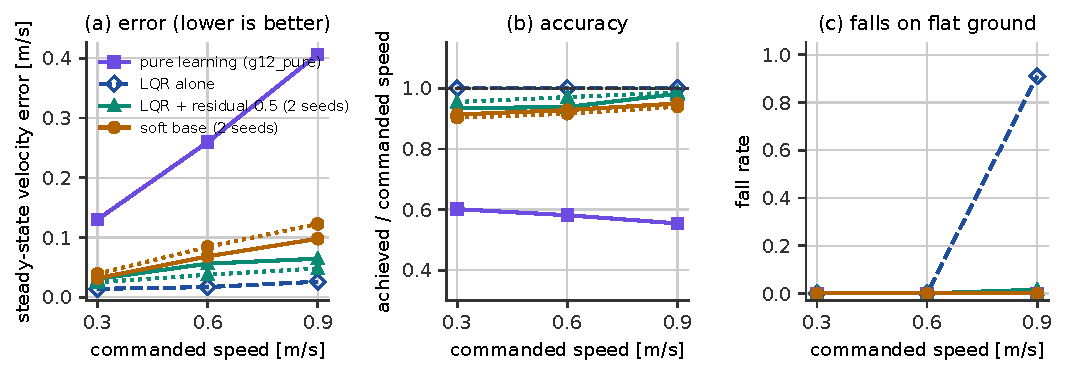
\includegraphics[width=\textwidth]{figures/study_tracking.pdf}
\caption{Tracking error, achieved/commanded speed and falls versus commanded speed. Engine: Warp GPU, corrected. Randomisation: off. Noise: off. Worlds per point: 64 (LQR alone: hollow markers; its error and ratio at 0.9\,m/s are over the few surviving worlds). Seeds: one for pure learning, two for the residual and the soft base (dotted). Protocol: clean flat benchmark of Table~\ref{tab:gen_flat}. Data files store means only, so no error bars.}\label{fig:tracking}
\end{figure*}

\subsection{Goal task and velocity task on the tiles}
On the goal task (Table~\ref{tab:gen_goal}, Fig.~\ref{fig:terraingoal}) the residual (A, two seeds) succeeds in \gv{fam.res.u.1} of undisturbed worlds in a median \gv{fam.res.time}\,s; pure learning in \gv{fam.pure.u.1} in \gv{fam.pure.time}\,s, and the soft base in \gv{fam.soft.u.1} in \gv{fam.soft.time}\,s. By kind the residual reaches the goal on ramps up in \gv{fam.res.k.ramp_up} of worlds, on flat tiles \gv{fam.res.k.flat}, stairs \gv{fam.res.k.stairs}, step ups \gv{fam.res.k.step_up} and bumps \gv{fam.res.k.bump}. With pushes and pulls success drops to 0.25 to 0.34 for every recipe, pure learning included (\gv{fam.pure.d.1}). On the velocity task at 0.3\,m/s on the tiles (Table~\ref{tab:gen_veltiles}) the residual falls in \gv{fam.res.velu} of worlds undisturbed and \gv{fam.res.veld} with pushes and pulls, and so do the ramped and soft recipes; pure learning has fewer falls (\gv{fam.pure.velu}, \gv{fam.pure.veld}) but tracks at about \gv{fam.pure.ratio03} of the command on the flat world, so this is not a robustness advantage.
\begin{table*}[t]\centering\footnotesize
\caption{Goal task on the tiled terrain, corrected engine. Engine: Warp GPU (MuJoCo-Warp 3.17, float32), corrected for the S69 stale-subtree-mass error. Domain randomisation: on at scale 1 (mass, friction, damping, torque, latency, floor classes, 11 designs). Observation noise: on. Worlds per cell: 16 per (design, terrain kind): 176 per terrain kind, 1760 per row. Seeds: one per row as listed. Protocol: goal 1.1 m from a random start on a tile, success = within 0.2 m before any fall within 800 steps (eval\_battery.py); terrain columns are undisturbed success per kind; undisturbed = pushes and pulls off, disturbed = pushes 5 to 20 N and pulls 3 to 12 N. g14 rows are one-variable changes of the ramped (B) or soft (C) recipe.}\label{tab:gen_goal}
\resizebox{\textwidth}{!}{%
\begin{tabular}{lccccccccc}\toprule
Policy & Undisturbed: falls / success & median time [s] & step up & stairs & bump & ramp up & flat & Pushes + pulls: falls / success & Seed\\\midrule
pure learning (no LQR), 300M steps g12\_pure\_s0, seed 0 & 0.32 / 0.44 & 3.08 & 0.19 & 0.14 & 0.19 & 0.23 & 0.73 & 0.62 / 0.26 & seed 0\\
LQR + residual 0.5, standard randomisation g12\_res\_s0, seed 0 & 0.42 / 0.58 & 2.61 & 0.33 & 0.38 & 0.17 & 0.74 & 0.84 & 0.75 / 0.25 & seed 0\\
LQR + residual 0.5, standard randomisation g12\_res\_s1, seed 1 & 0.42 / 0.58 & 2.43 & 0.28 & 0.39 & 0.20 & 0.69 & 0.82 & 0.73 / 0.27 & seed 1\\
LQR + residual 0.5, randomisation ramped to 1.75x g12\_dr175\_s0, seed 0 & 0.42 / 0.58 & 2.44 & 0.31 & 0.44 & 0.26 & 0.65 & 0.80 & 0.71 / 0.29 & seed 0\\
LQR + residual 0.5, randomisation ramped to 1.75x g12\_dr175\_s1, seed 1 & 0.40 / 0.60 & 2.33 & 0.39 & 0.47 & 0.20 & 0.69 & 0.81 & 0.70 / 0.30 & seed 1\\
soft LQR base (R x3, a\_max 0.3), ramped to 1.75x g12\_soft175\_s0, seed 0 & 0.37 / 0.63 & 3.06 & 0.35 & 0.39 & 0.16 & 0.75 & 0.87 & 0.67 / 0.33 & seed 0\\
soft LQR base (R x3, a\_max 0.3), ramped to 1.75x g12\_soft175\_s1, seed 1 & 0.38 / 0.62 & 3.12 & 0.28 & 0.34 & 0.18 & 0.74 & 0.89 & 0.66 / 0.34 & seed 1\\
soft LQR base, authority 0.75 g13\_softrs075\_s0, seed 0 & 0.42 / 0.58 & 3.37 & 0.22 & 0.26 & 0.15 & 0.67 & 0.84 & 0.68 / 0.32 & seed 0\\
ramped 1.75x, fall penalty 5 (was 2) g14\_fp5\_s0, seed 0 & 0.43 / 0.57 & 2.41 & 0.32 & 0.38 & 0.19 & 0.70 & 0.80 & 0.73 / 0.27 & seed 0\\
soft base, fall penalty 5 g14\_softfp5\_s0, seed 0 & 0.37 / 0.63 & 2.98 & 0.35 & 0.32 & 0.18 & 0.77 & 0.89 & 0.67 / 0.33 & seed 0\\
ramped 1.75x, push and pull strength ramped 0.2 to 1 g14\_pramp\_s0, seed 0 & 0.43 / 0.57 & 2.29 & 0.34 & 0.37 & 0.18 & 0.66 & 0.79 & 0.75 / 0.25 & seed 0\\
ramped 1.75x + edge starts + depth sensor g15\_edge\_depth\_s0, seed 0 & 0.40 / 0.60 & 2.36 & 0.36 & 0.44 & 0.27 & 0.66 & 0.80 & 0.71 / 0.29 & seed 0\\
ramped 1.75x + edge starts, blind control g15\_edge\_blind\_s0, seed 0 & 0.40 / 0.60 & 2.30 & 0.38 & 0.41 & 0.28 & 0.65 & 0.80 & 0.72 / 0.28 & seed 0\\
pure learning (no LQR), 300M steps g12\_pure\_s1, seed 1 & 0.36 / 0.51 & 2.97 & 0.26 & 0.27 & 0.26 & 0.28 & 0.80 & 0.66 / 0.27 & seed 1\\
ramped 1.75x, trained with the ball retainer (arrestors at 100 deg) g16\_ret100\_s0, seed 0 & 0.28 / 0.71 & 2.81 & 0.47 & 0.52 & 0.40 & 0.76 & 0.88 & 0.53 / 0.46 & seed 0\\
ramped 1.75x, trained with the ball retainer (arrestors at 100 deg) g16\_ret100\_s1, seed 1 & 0.24 / 0.76 & 2.75 & 0.55 & 0.64 & 0.51 & 0.86 & 0.89 & 0.51 / 0.49 & seed 1\\
pure learning, trained with the retainer g16\_pure\_ret100\_s0, seed 0 & 0.14 / 0.70 & 2.96 & 0.42 & 0.35 & 0.44 & 0.56 & 0.95 & 0.40 / 0.50 & seed 0\\
pure learning, trained with the retainer g16\_pure\_ret100\_s1, seed 1 & 0.15 / 0.74 & 2.62 & 0.58 & 0.55 & 0.53 & 0.65 & 0.88 & 0.44 / 0.50 & seed 1\\
retainer, authority 0.5, tracking weight x3 g17\_ret100\_trk3\_s0, seed 0 & 0.28 / 0.71 & 3.10 & 0.47 & 0.60 & 0.35 & 0.81 & 0.89 & 0.51 / 0.49 & seed 0\\
retainer, authority 0.15 g18\_ret\_rs015\_s0, seed 0 & 0.31 / 0.69 & 2.24 & 0.48 & 0.57 & 0.44 & 0.75 & 0.81 & 0.65 / 0.35 & seed 0\\
retainer, authority 0.25 (recommended) g18\_ret\_rs025\_s0, seed 0 & 0.28 / 0.71 & 2.44 & 0.52 & 0.57 & 0.49 & 0.83 & 0.84 & 0.58 / 0.42 & seed 0\\
retainer, authority 0.25 (recommended) g18\_ret\_rs025\_s1, seed 1 & 0.24 / 0.76 & 2.50 & 0.56 & 0.62 & 0.54 & 0.84 & 0.88 & 0.57 / 0.43 & seed 1\\
retainer, authority 0.35 g18\_ret\_rs035\_s0, seed 0 & 0.28 / 0.72 & 2.73 & 0.50 & 0.60 & 0.45 & 0.81 & 0.88 & 0.55 / 0.45 & seed 0\\
retainer, soft LQR base, authority 0.5 g18\_ret\_soft\_s0, seed 0 & 0.24 / 0.75 & 2.96 & 0.51 & 0.55 & 0.39 & 0.84 & 0.93 & 0.49 / 0.51 & seed 0\\
retainer, authority 0.25 (recommended) g18\_ret\_rs025\_s2, seed 2 & 0.24 / 0.76 & 2.68 & 0.56 & 0.65 & 0.49 & 0.86 & 0.87 & 0.56 / 0.44 & seed 2\\
retainer, authority 0.25, 400M steps g19\_ret\_rs025\_400m\_s0, seed 0 & 0.25 / 0.75 & 2.61 & 0.52 & 0.63 & 0.49 & 0.86 & 0.87 & 0.57 / 0.43 & seed 0\\
retainer, authority 0.25, depth sensor + edge starts g20\_ret\_rs025\_depth\_s0, seed 0 & 0.26 / 0.74 & 2.52 & 0.56 & 0.61 & 0.50 & 0.85 & 0.86 & 0.57 / 0.43 & seed 0\\
retainer, authority 0.25, 12 training designs (adds tau3; 1920 worlds per goal row) g21\_ret\_rs025\_tau3\_s0, seed 0 & 0.29 / 0.71 & 2.51 & 0.51 & 0.64 & 0.52 & 0.83 & 0.82 & 0.59 / 0.41 & seed 0\\
retainer, authority 0.25, 12 training designs (adds tau3; 1920 worlds per goal row) g21\_ret\_rs025\_tau3\_s1, seed 1 & 0.33 / 0.67 & 2.54 & 0.47 & 0.54 & 0.43 & 0.79 & 0.80 & 0.60 / 0.40 & seed 1\\
retainer, authority 0.25, privileged height scan input g22\_ret\_rs025\_scan\_s0, seed 0 & 0.32 / 0.68 & 2.56 & 0.49 & 0.55 & 0.45 & 0.72 & 0.81 & 0.59 / 0.41 & seed 0\\
retainer, authority 0.5, privileged height scan input g22\_ret\_rs05\_scan\_s0, seed 0 & 0.26 / 0.74 & 2.86 & 0.50 & 0.61 & 0.41 & 0.84 & 0.87 & 0.47 / 0.53 & seed 0\\
pure learning, retainer, privileged height scan input g22\_pure\_ret\_scan\_s0, seed 0 & 0.17 / 0.69 & 2.96 & 0.47 & 0.42 & 0.32 & 0.44 & 0.93 & 0.40 / 0.50 & seed 0\\
recommended recipe on the corrected contact model (free-rolling friction 0.01; recommended checkpoint) g26\_ret\_rs025\_mu01\_s0, seed 0 & 0.26 / 0.74 & 2.62 & 0.52 & 0.65 & 0.40 & 0.85 & 0.89 & 0.55 / 0.45 & seed 0\\
recommended recipe on the corrected contact model (free-rolling friction 0.01; recommended checkpoint) g26\_ret\_rs025\_mu01\_s1, seed 1 & 0.26 / 0.74 & 2.67 & 0.52 & 0.61 & 0.42 & 0.86 & 0.88 & 0.54 / 0.46 & seed 1\\
recommended recipe on the corrected contact model (free-rolling friction 0.01; recommended checkpoint) g26\_ret\_rs025\_mu01\_s2, seed 2 & 0.27 / 0.73 & 2.58 & 0.53 & 0.64 & 0.41 & 0.86 & 0.88 & 0.55 / 0.45 & seed 2\\
recommended recipe, trained with the planner in the loop (30 \% of worlds on blocks tiles) g23\_nav\_rs025\_s0, seed 0 & 0.29 / 0.71 & 2.82 & 0.47 & 0.57 & 0.41 & 0.85 & 0.85 & 0.57 / 0.43 & seed 0\\
recommended recipe, trained with the planner in the loop (30 \% of worlds on blocks tiles) g23\_nav\_rs025\_s1, seed 1 & 0.30 / 0.70 & 2.55 & 0.52 & 0.56 & 0.44 & 0.81 & 0.84 & 0.57 / 0.43 & seed 1\\
\bottomrule\end{tabular}}
\end{table*}

\begin{table}[t]\centering\footnotesize
\caption{Velocity task at 0.3\,m/s on the tiled terrain, corrected engine. Engine: Warp GPU (MuJoCo-Warp 3.17, float32), corrected for the S69 stale-subtree-mass error. Domain randomisation: on at scale 1. Observation noise: on. Worlds per cell: 16 per (design, terrain kind): 1760 per cell. Seeds: one per row as listed. Protocol: velocity task at 0.3 m/s at a random heading on the tiles with floor classes, 800 steps (eval\_battery.py); tracking error is the mean over upright steps.}\label{tab:gen_veltiles}
\resizebox{\columnwidth}{!}{%
\begin{tabular}{lcccc}\toprule
Policy & Falls, undisturbed & Falls, pushes + pulls & Tracking error undisturbed / disturbed [m/s] & Seed\\\midrule
pure learning (no LQR), 300M steps g12\_pure\_s0, seed 0 & 0.32 & 0.54 & 0.194 / 0.292 & seed 0\\
LQR + residual 0.5, standard randomisation g12\_res\_s0, seed 0 & 0.55 & 0.72 & 0.112 / 0.218 & seed 0\\
LQR + residual 0.5, standard randomisation g12\_res\_s1, seed 1 & 0.55 & 0.74 & 0.104 / 0.205 & seed 1\\
LQR + residual 0.5, randomisation ramped to 1.75x g12\_dr175\_s0, seed 0 & 0.54 & 0.71 & 0.109 / 0.217 & seed 0\\
LQR + residual 0.5, randomisation ramped to 1.75x g12\_dr175\_s1, seed 1 & 0.53 & 0.71 & 0.102 / 0.226 & seed 1\\
soft LQR base (R x3, a\_max 0.3), ramped to 1.75x g12\_soft175\_s0, seed 0 & 0.55 & 0.71 & 0.109 / 0.208 & seed 0\\
soft LQR base (R x3, a\_max 0.3), ramped to 1.75x g12\_soft175\_s1, seed 1 & 0.53 & 0.73 & 0.118 / 0.212 & seed 1\\
soft LQR base, authority 0.75 g13\_softrs075\_s0, seed 0 & 0.54 & 0.70 & 0.123 / 0.217 & seed 0\\
ramped 1.75x, fall penalty 5 (was 2) g14\_fp5\_s0, seed 0 & 0.54 & 0.73 & 0.110 / 0.219 & seed 0\\
soft base, fall penalty 5 g14\_softfp5\_s0, seed 0 & 0.54 & 0.71 & 0.113 / 0.223 & seed 0\\
ramped 1.75x, push and pull strength ramped 0.2 to 1 g14\_pramp\_s0, seed 0 & 0.54 & 0.73 & 0.111 / 0.222 & seed 0\\
ramped 1.75x + edge starts + depth sensor g15\_edge\_depth\_s0, seed 0 & 0.56 & 0.73 & 0.101 / 0.223 & seed 0\\
ramped 1.75x + edge starts, blind control g15\_edge\_blind\_s0, seed 0 & 0.53 & 0.73 & 0.105 / 0.228 & seed 0\\
pure learning (no LQR), 300M steps g12\_pure\_s1, seed 1 & 0.38 & 0.57 & 0.181 / 0.274 & seed 1\\
ramped 1.75x, trained with the ball retainer (arrestors at 100 deg) g16\_ret100\_s0, seed 0 & 0.31 & 0.49 & 0.141 / 0.226 & seed 0\\
ramped 1.75x, trained with the ball retainer (arrestors at 100 deg) g16\_ret100\_s1, seed 1 & 0.32 & 0.50 & 0.138 / 0.220 & seed 1\\
pure learning, trained with the retainer g16\_pure\_ret100\_s0, seed 0 & 0.16 & 0.34 & 0.171 / 0.251 & seed 0\\
pure learning, trained with the retainer g16\_pure\_ret100\_s1, seed 1 & 0.19 & 0.38 & 0.155 / 0.235 & seed 1\\
retainer, authority 0.5, tracking weight x3 g17\_ret100\_trk3\_s0, seed 0 & 0.32 & 0.46 & 0.141 / 0.219 & seed 0\\
retainer, authority 0.15 g18\_ret\_rs015\_s0, seed 0 & 0.38 & 0.58 & 0.126 / 0.246 & seed 0\\
retainer, authority 0.25 (recommended) g18\_ret\_rs025\_s0, seed 0 & 0.34 & 0.55 & 0.125 / 0.235 & seed 0\\
retainer, authority 0.25 (recommended) g18\_ret\_rs025\_s1, seed 1 & 0.35 & 0.56 & 0.131 / 0.236 & seed 1\\
retainer, authority 0.35 g18\_ret\_rs035\_s0, seed 0 & 0.34 & 0.52 & 0.132 / 0.223 & seed 0\\
retainer, soft LQR base, authority 0.5 g18\_ret\_soft\_s0, seed 0 & 0.29 & 0.49 & 0.150 / 0.217 & seed 0\\
retainer, authority 0.25 (recommended) g18\_ret\_rs025\_s2, seed 2 & 0.36 & 0.55 & 0.137 / 0.224 & seed 2\\
retainer, authority 0.25, 400M steps g19\_ret\_rs025\_400m\_s0, seed 0 & 0.38 & 0.55 & 0.140 / 0.221 & seed 0\\
retainer, authority 0.25, depth sensor + edge starts g20\_ret\_rs025\_depth\_s0, seed 0 & 0.35 & 0.54 & 0.121 / 0.224 & seed 0\\
retainer, authority 0.25, 12 training designs (adds tau3; 1920 worlds per goal row) g21\_ret\_rs025\_tau3\_s0, seed 0 & 0.35 & 0.56 & 0.127 / 0.232 & seed 0\\
retainer, authority 0.25, 12 training designs (adds tau3; 1920 worlds per goal row) g21\_ret\_rs025\_tau3\_s1, seed 1 & 0.36 & 0.57 & 0.130 / 0.228 & seed 1\\
retainer, authority 0.25, privileged height scan input g22\_ret\_rs025\_scan\_s0, seed 0 & 0.36 & 0.55 & 0.132 / 0.226 & seed 0\\
retainer, authority 0.5, privileged height scan input g22\_ret\_rs05\_scan\_s0, seed 0 & 0.32 & 0.48 & 0.131 / 0.213 & seed 0\\
pure learning, retainer, privileged height scan input g22\_pure\_ret\_scan\_s0, seed 0 & 0.15 & 0.35 & 0.165 / 0.231 & seed 0\\
recommended recipe on the corrected contact model (free-rolling friction 0.01; recommended checkpoint) g26\_ret\_rs025\_mu01\_s0, seed 0 & 0.34 & 0.53 & 0.134 / 0.220 & seed 0\\
recommended recipe on the corrected contact model (free-rolling friction 0.01; recommended checkpoint) g26\_ret\_rs025\_mu01\_s1, seed 1 & 0.34 & 0.51 & 0.140 / 0.229 & seed 1\\
recommended recipe on the corrected contact model (free-rolling friction 0.01; recommended checkpoint) g26\_ret\_rs025\_mu01\_s2, seed 2 & 0.34 & 0.53 & 0.138 / 0.227 & seed 2\\
recommended recipe, trained with the planner in the loop (30 \% of worlds on blocks tiles) g23\_nav\_rs025\_s0, seed 0 & 0.36 & 0.55 & 0.132 / 0.204 & seed 0\\
recommended recipe, trained with the planner in the loop (30 \% of worlds on blocks tiles) g23\_nav\_rs025\_s1, seed 1 & 0.36 & 0.55 & 0.126 / 0.213 & seed 1\\
\bottomrule\end{tabular}}
\end{table}

\begin{figure}[t]\centering
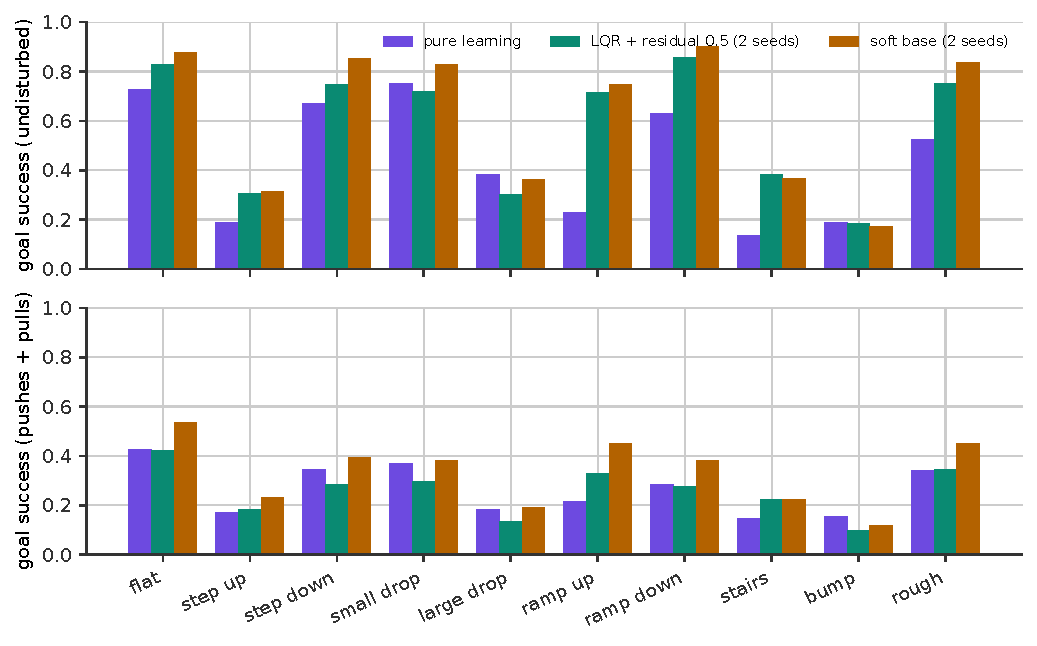
\includegraphics[width=\columnwidth]{figures/study_terrain_goal.pdf}
\caption{Goal success per terrain kind, undisturbed (top) and with pushes and pulls (bottom). Engine: Warp GPU, corrected. Randomisation: on at scale 1. Noise: on. Worlds per bar: 176. Seeds: one for pure learning, two averaged otherwise. Protocol: goal task of Table~\ref{tab:gen_goal}.}\label{fig:terraingoal}
\end{figure}

\subsection{Soft base, authority and seed noise}
The soft base gives a small, consistent gain in goal success (+\gv{cmp.soft_gain_u} undisturbed, +\gv{cmp.soft_gain_d} with pushes and pulls at scale 1) at the cost of speed (\gv{fam.soft.time}\,s against \gv{fam.res.time}\,s) and a little flat accuracy at 0.9\,m/s (error \gvt{fam.soft.flat09} against \gvt{fam.res.flat09}\,m/s). Authority 0.75 on the soft base is no better (goal success \gv{goal.g13_softrs075_s0.u.success}) and tracks worse on the flat floor (error \gvt{flat.g13_softrs075_s0.0.9.err}, falls \gv{flat.g13_softrs075_s0.0.9.fall} at 0.9\,m/s; Fig.~\ref{fig:authority}). Seed replicates agree: goal success differs by at most \gv{seeds.goal_maxdiff} at every randomisation scale and with or without disturbances (Fig.~\ref{fig:seeds}).
\begin{figure*}[t]\centering
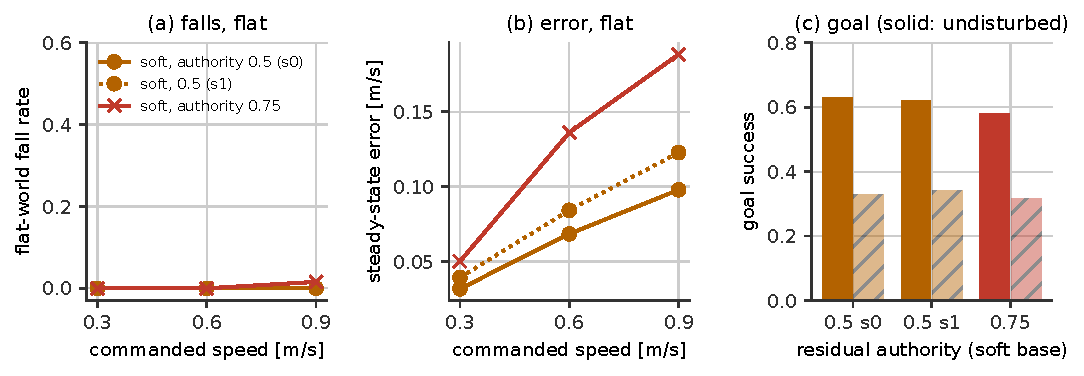
\includegraphics[width=\textwidth]{figures/study_authority.pdf}
\caption{Authority 0.5 against 0.75 on the soft base. Engine: Warp GPU, corrected. Randomisation: off in (a, b), on at scale 1 in (c). Noise: off (a, b), on (c). Worlds: 64 per point (a, b), 1760 per bar (c; solid undisturbed, hatched with pushes and pulls). Seeds: two at 0.5, one at 0.75. Protocol: Tables~\ref{tab:gen_flat} and~\ref{tab:gen_goal}.}\label{fig:authority}
\end{figure*}
\begin{figure}[t]\centering
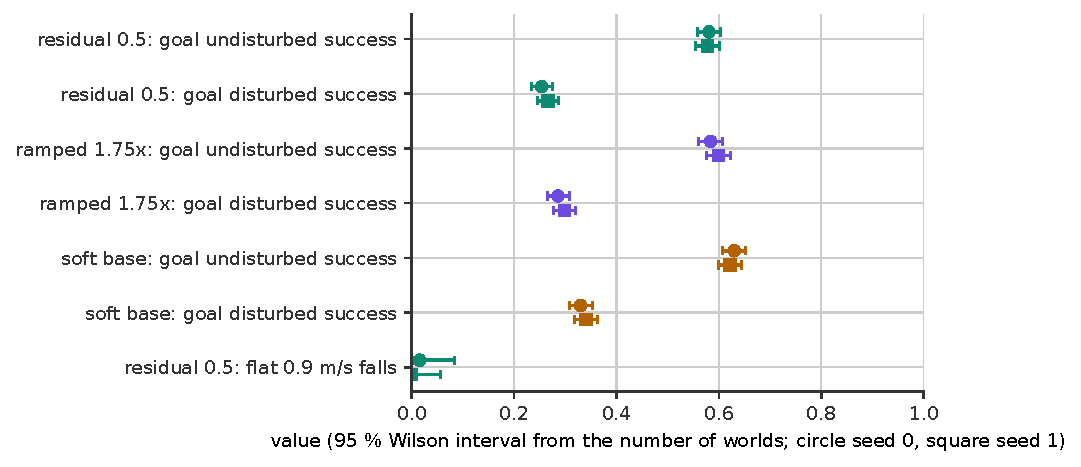
\includegraphics[width=0.95\columnwidth]{figures/study_seeds.pdf}
\caption{Seed noise. Engine: Warp GPU, corrected. Randomisation: on at scale 1 (flat row: off). Noise: on (flat row: off). Worlds: 1760 per point (flat row: 64). Seeds: two per recipe, circle seed 0, square seed 1. Bars are 95\,\% Wilson intervals for sampling of worlds only.}\label{fig:seeds}
\end{figure}

\subsection{Robustness to randomisation and disturbances}
Evaluated at randomisation scales 1, 1.75 and 2.5 (Table~\ref{tab:gen_robust}, Fig.~\ref{fig:robustrun}), goal success falls from \gv{fam.res.u.1} to \gv{fam.res.u.2.5} for the standard-range policy; training over the 1.75 times ranges changes it by at most \gv{cmp.dr_gain_u} undisturbed and \gv{cmp.dr_gain_d} with pushes and pulls, within seed noise, so the standard-range policy is already robust to wider parameter ranges, and pure learning degrades alike (\gv{fam.pure.u.1} to \gv{fam.pure.u.2.5}). What no recipe changes is the success under pushes and pulls (about 0.3) and the tile velocity falls. Three disturbance-focused one-variable changes (fall penalty 5 on the ramped recipe, fall penalty 5 on the soft base, push and pull strength ramped from 0.2 to 1 in training) were also evaluated: \emph{none improved robustness under pushes and pulls} (goal success \gv{goal.g14_fp5_s0.d.success}, \gv{goal.g14_softfp5_s0.d.success} and \gv{goal.g14_pramp_s0.d.success} at scale 1 against \gv{fam.dr175.d.1} for the ramped recipe and \gv{fam.soft.d.1} for the soft base); the push curriculum is slightly worse. On a held-out terrain layout (tile seed 1, Table~\ref{tab:gen_heldout}) the ramped recipe reaches \gv{held.g12_dr175_s0.u} and \gv{held.g12_dr175_s1.u} undisturbed and \gv{held.g12_dr175_s0.d} and \gv{held.g12_dr175_s1.d} disturbed on two seeds, a small drop from the trained map. \tbd{privileged height scan on the corrected engine and second seeds of the perception arms.}
\begin{table*}[t]\centering\footnotesize
\caption{Goal success against randomisation scale, corrected engine. Engine: Warp GPU (MuJoCo-Warp 3.17, float32), corrected for the S69 stale-subtree-mass error. Domain randomisation: on; evaluated at the scale in the column (policies trained at scale 1 or ramped to 1.75). Observation noise: on. Worlds per cell: 1760 per cell. Seeds: one per row as listed. Protocol: goal task of Table 2 at DR scales 1, 1.75 and 2.5 (the master scale multiplies mass, friction, torque, damping, latency and noise ranges, not push or pull strength).}\label{tab:gen_robust}
\resizebox{\textwidth}{!}{%
\begin{tabular}{lccccc}\toprule
Policy & Goal success, DR 1: undisturbed / disturbed & DR 1.75 & DR 2.5 & Tile velocity falls, DR 2.5 undisturbed & Seed\\\midrule
pure learning (no LQR), 300M steps g12\_pure\_s0, seed 0 & 0.44 / 0.26 & 0.43 / 0.23 & 0.37 / 0.18 & 0.52 & seed 0\\
LQR + residual 0.5, standard randomisation g12\_res\_s0, seed 0 & 0.58 / 0.25 & 0.52 / 0.23 & 0.45 / 0.18 & 0.66 & seed 0\\
LQR + residual 0.5, standard randomisation g12\_res\_s1, seed 1 & 0.58 / 0.27 & 0.54 / 0.25 & 0.44 / 0.19 & 0.65 & seed 1\\
LQR + residual 0.5, randomisation ramped to 1.75x g12\_dr175\_s0, seed 0 & 0.58 / 0.29 & 0.54 / 0.25 & 0.45 / 0.19 & 0.62 & seed 0\\
LQR + residual 0.5, randomisation ramped to 1.75x g12\_dr175\_s1, seed 1 & 0.60 / 0.30 & 0.56 / 0.25 & 0.47 / 0.19 & 0.62 & seed 1\\
soft LQR base (R x3, a\_max 0.3), ramped to 1.75x g12\_soft175\_s0, seed 0 & 0.63 / 0.33 & 0.57 / 0.29 & 0.49 / 0.23 & 0.65 & seed 0\\
soft LQR base (R x3, a\_max 0.3), ramped to 1.75x g12\_soft175\_s1, seed 1 & 0.62 / 0.34 & 0.58 / 0.29 & 0.52 / 0.24 & 0.63 & seed 1\\
soft LQR base, authority 0.75 g13\_softrs075\_s0, seed 0 & 0.58 / 0.32 & 0.53 / 0.26 & 0.45 / 0.21 & 0.66 & seed 0\\
ramped 1.75x, fall penalty 5 (was 2) g14\_fp5\_s0, seed 0 & 0.57 / 0.27 & 0.53 / 0.25 & 0.46 / 0.18 & 0.63 & seed 0\\
soft base, fall penalty 5 g14\_softfp5\_s0, seed 0 & 0.63 / 0.33 & 0.59 / 0.27 & 0.50 / 0.22 & 0.65 & seed 0\\
ramped 1.75x, push and pull strength ramped 0.2 to 1 g14\_pramp\_s0, seed 0 & 0.57 / 0.25 & 0.52 / 0.21 & 0.47 / 0.16 & 0.62 & seed 0\\
ramped 1.75x + edge starts + depth sensor g15\_edge\_depth\_s0, seed 0 & 0.60 / 0.29 & 0.53 / 0.26 & 0.45 / 0.18 & 0.64 & seed 0\\
ramped 1.75x + edge starts, blind control g15\_edge\_blind\_s0, seed 0 & 0.60 / 0.28 & 0.54 / 0.23 & 0.47 / 0.19 & 0.61 & seed 0\\
pure learning (no LQR), 300M steps g12\_pure\_s1, seed 1 & 0.51 / 0.27 & 0.44 / 0.23 & 0.39 / 0.19 & 0.58 & seed 1\\
ramped 1.75x, trained with the ball retainer (arrestors at 100 deg) g16\_ret100\_s0, seed 0 & 0.71 / 0.46 & 0.70 / 0.42 & 0.62 / 0.35 & 0.42 & seed 0\\
ramped 1.75x, trained with the ball retainer (arrestors at 100 deg) g16\_ret100\_s1, seed 1 & 0.76 / 0.49 & 0.73 / 0.44 & 0.67 / 0.37 & 0.44 & seed 1\\
pure learning, trained with the retainer g16\_pure\_ret100\_s0, seed 0 & 0.70 / 0.50 & 0.67 / 0.45 & 0.64 / 0.40 & 0.29 & seed 0\\
pure learning, trained with the retainer g16\_pure\_ret100\_s1, seed 1 & 0.74 / 0.50 & 0.73 / 0.46 & 0.67 / 0.40 & 0.33 & seed 1\\
retainer, authority 0.5, tracking weight x3 g17\_ret100\_trk3\_s0, seed 0 & 0.71 / 0.49 & 0.68 / 0.43 & 0.62 / 0.36 & 0.44 & seed 0\\
retainer, authority 0.15 g18\_ret\_rs015\_s0, seed 0 & 0.69 / 0.35 & 0.65 / 0.31 & 0.56 / 0.22 & 0.45 & seed 0\\
retainer, authority 0.25 (recommended) g18\_ret\_rs025\_s0, seed 0 & 0.71 / 0.42 & 0.68 / 0.36 & 0.60 / 0.29 & 0.44 & seed 0\\
retainer, authority 0.25 (recommended) g18\_ret\_rs025\_s1, seed 1 & 0.76 / 0.43 & 0.72 / 0.39 & 0.66 / 0.32 & 0.46 & seed 1\\
retainer, authority 0.35 g18\_ret\_rs035\_s0, seed 0 & 0.72 / 0.45 & 0.71 / 0.40 & 0.63 / 0.32 & 0.44 & seed 0\\
retainer, soft LQR base, authority 0.5 g18\_ret\_soft\_s0, seed 0 & 0.75 / 0.51 & 0.75 / 0.47 & 0.66 / 0.39 & 0.44 & seed 0\\
retainer, authority 0.25 (recommended) g18\_ret\_rs025\_s2, seed 2 & 0.76 / 0.44 & 0.71 / 0.41 & 0.63 / 0.32 & 0.46 & seed 2\\
retainer, authority 0.25, 400M steps g19\_ret\_rs025\_400m\_s0, seed 0 & 0.75 / 0.43 & 0.70 / 0.36 & 0.64 / 0.30 & 0.48 & seed 0\\
retainer, authority 0.25, depth sensor + edge starts g20\_ret\_rs025\_depth\_s0, seed 0 & 0.74 / 0.43 & 0.69 / 0.38 & 0.63 / 0.31 & 0.46 & seed 0\\
retainer, authority 0.25, 12 training designs (adds tau3; 1920 worlds per goal row) g21\_ret\_rs025\_tau3\_s0, seed 0 & 0.71 / 0.41 & 0.66 / 0.36 & 0.58 / 0.29 & 0.45 & seed 0\\
retainer, authority 0.25, 12 training designs (adds tau3; 1920 worlds per goal row) g21\_ret\_rs025\_tau3\_s1, seed 1 & 0.67 / 0.40 & 0.63 / 0.34 & 0.56 / 0.26 & 0.49 & seed 1\\
retainer, authority 0.25, privileged height scan input g22\_ret\_rs025\_scan\_s0, seed 0 & 0.68 / 0.41 & 0.64 / 0.35 & 0.56 / 0.28 & 0.47 & seed 0\\
retainer, authority 0.5, privileged height scan input g22\_ret\_rs05\_scan\_s0, seed 0 & 0.74 / 0.53 & 0.71 / 0.48 & 0.65 / 0.36 & 0.46 & seed 0\\
pure learning, retainer, privileged height scan input g22\_pure\_ret\_scan\_s0, seed 0 & 0.69 / 0.50 & 0.67 / 0.46 & 0.64 / 0.40 & 0.31 & seed 0\\
recommended recipe on the corrected contact model (free-rolling friction 0.01; recommended checkpoint) g26\_ret\_rs025\_mu01\_s0, seed 0 & 0.74 / 0.45 & 0.72 / 0.41 & 0.68 / 0.33 & 0.38 & seed 0\\
recommended recipe on the corrected contact model (free-rolling friction 0.01; recommended checkpoint) g26\_ret\_rs025\_mu01\_s1, seed 1 & 0.74 / 0.46 & 0.72 / 0.42 & 0.69 / 0.36 & 0.39 & seed 1\\
recommended recipe on the corrected contact model (free-rolling friction 0.01; recommended checkpoint) g26\_ret\_rs025\_mu01\_s2, seed 2 & 0.73 / 0.45 & 0.72 / 0.41 & 0.68 / 0.34 & 0.39 & seed 2\\
recommended recipe, trained with the planner in the loop (30 \% of worlds on blocks tiles) g23\_nav\_rs025\_s0, seed 0 & 0.71 / 0.43 & 0.67 / 0.39 & 0.61 / 0.31 & 0.46 & seed 0\\
recommended recipe, trained with the planner in the loop (30 \% of worlds on blocks tiles) g23\_nav\_rs025\_s1, seed 1 & 0.70 / 0.43 & 0.67 / 0.40 & 0.59 / 0.30 & 0.46 & seed 1\\
\bottomrule\end{tabular}}
\end{table*}

\begin{table*}[t]\centering\footnotesize
\caption{Goal task on held-out terrain (tile seed 1), corrected engine. Engine: Warp GPU (MuJoCo-Warp 3.17, float32), corrected for the S69 stale-subtree-mass error. Domain randomisation: on at scale 1. Observation noise: on. Worlds per cell: 16 per (design, terrain kind): 176 per terrain kind, 1760 per cell. Seeds: seeds 0 and 1 of the recipe. Protocol: goal task of Table 2 on a freshly generated tile map (tile seed 1: new severities and positions, same ten kinds and ranges) while the policy was trained on tile seed 0; undisturbed = pushes and pulls off, disturbed = on.}\label{tab:gen_heldout}
\resizebox{\textwidth}{!}{%
\begin{tabular}{lcccccc}\toprule
Policy & Undisturbed success, tile seed 1 (held out) & tile seed 0 (trained) & Disturbed success, tile seed 1 & tile seed 0 & Median time [s], undisturbed / disturbed & Seed\\\midrule
ramped to 1.75x (g12\_dr175\_s0, seed 0) & 0.52 & 0.58 & 0.26 & 0.29 & 2.44 / 2.35 & seed 0\\
ramped to 1.75x (g12\_dr175\_s1, seed 1) & 0.53 & 0.60 & 0.26 & 0.30 & 2.32 / 2.24 & seed 1\\
\bottomrule\end{tabular}}
\end{table*}

\begin{figure}[t]\centering
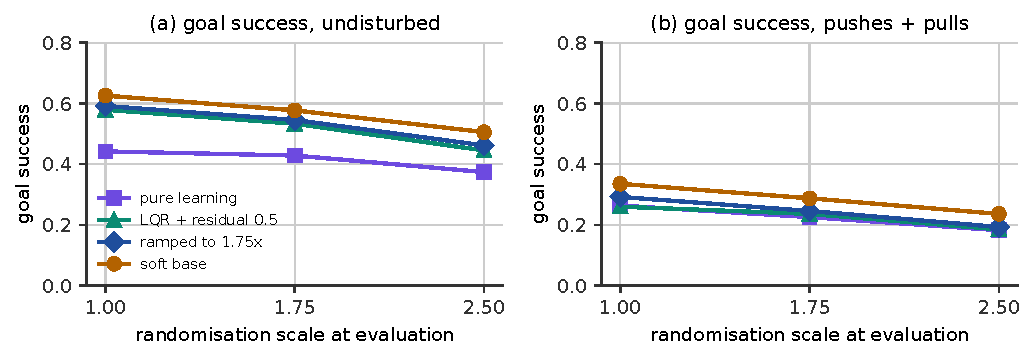
\includegraphics[width=\columnwidth]{figures/study_robust.pdf}
\caption{Goal success against randomisation scale. Engine: Warp GPU, corrected. Randomisation: on, at the scale on the axis. Noise: on. Worlds: 1760 per point. Seeds: one for pure learning, two averaged for the others. Protocol: goal task, undisturbed (a) and with pushes and pulls (b).}\label{fig:robustrun}
\end{figure}

\subsection{Why it falls, and a ball retainer}\label{sec:retainer}
\paragraph{Fall diagnosis.} The simulated robot is two free bodies, the base (with the wheels) and the ball, held together only by gravity and the three wheel-ball contacts. Logging every world at every step for the ramped policy (Table~\ref{tab:gen_fallcause}) shows that the motors do not run out of torque (wheels at the limit for \gv{fc.u.sat}\,\% of the last second before an undisturbed fall, \gv{fc.d.sat}\,\% with pushes and pulls) and that the robot rarely tips past 70$^\circ$ (\gv{fc.u.offset} of undisturbed falls end at the ball-offset limit). In \gv{fc.u.unseat} of undisturbed falls the body first derails off the ball (the base axis turns more than 5$^\circ$ away from the ball-centre-to-base direction, against 0.1 to 0.3$^\circ$ when seated) at a median tilt of only \gv{fc.u.tilt}$^\circ$; survivors reach about \gv{fc.u.surv}$^\circ$ without derailing.
\begin{table*}[t]\centering\footnotesize
\caption{Fall diagnosis, corrected engine. Engine: Warp GPU (MuJoCo-Warp 3.17, float32), corrected for the S69 stale-subtree-mass error. Domain randomisation: on at scale 1. Observation noise: on. Worlds per cell: 1760 (16 per design and terrain kind). Seeds: one policy (g12\_dr175\_s0, seed 0). Protocol: goal task of Table 2 with per-step logging (fall\_cause.py); derailed = the base axis is misaligned with the ball-centre-to-base direction by more than 5 deg (0.1 to 0.3 deg while the wheels sit on the ball).}\label{tab:gen_fallcause}
\resizebox{\textwidth}{!}{%
\begin{tabular}{lcccccc}\toprule
Condition & Fall rate & Falls ended by the ball-offset limit (tilt below 70 deg) & Body derailed before tipping & Median tilt when derailing [deg] & Wheels at the torque limit, last 1 s before the fall & Falls with a pull active\\\midrule
undisturbed & 0.43 & 0.95 & 0.78 & 14.7 & 0.7 \% & 0.00\\
pushes + pulls & 0.72 & 0.97 & 0.49 & 15.4 & 0.4 \% & 0.58\\
pushes + pulls, LQR alone (no residual) & 0.85 & 0.98 & 0.98 & not recorded & 0.4 \% & 0.71\\
\bottomrule\end{tabular}}
\end{table*}


\paragraph{Retainer design.} The idea is taken from the arrestors of ETH Zurich's Rezero ballbot, which according to its project coverage hold the ball against the wheels; no design details were published, so the design is our own. Three passive spherical arrestors of radius $r_a=8$\,mm are fixed to the base, one per wheel on the azimuth opposite that wheel, at polar angle $\phi$ from the top of the ball, with centres $\boldsymbol a_k=\boldsymbol c+(R+r_a)\,\boldsymbol u_k(\phi)$ computed at the \emph{loaded seat} (the model settled under gravity, about 1\,cm above the reset pose), so they touch the ball without preload, carry no force while the robot is seated, and act only when the body starts to lift or slide (Fig.~\ref{fig:retgeom}). A frictionless sphere-sphere contact force acts along the line of centres, $\boldsymbol F_k=\lambda_k\hat{\boldsymbol r}_k$ with $\boldsymbol r_k$ from the ball centre to the contact point and $\lambda_k\ge0$, so
\begin{equation}
\boldsymbol M_c=\sum_k\boldsymbol r_k\times\lambda_k\hat{\boldsymbol r}_k=\boldsymbol 0 .
\end{equation}
Such a force does no virtual work on the ball rotation $\varphi$ of the planar model, and $\lambda_k=0$ while seated; when an arrestor engages it only enforces the constraint the model already assumes (the body stays on the ball). The equations of motion, $(A,B_s)$ and the LQR gain are therefore unchanged. Roller friction $\mu$ adds a moment of at most $\mu\lambda_kR$, which is zero while seated (Table~\ref{tab:gen_friction}). With the robot upright the bottom of an arrestor sits $R+(R+r_a)\cos\phi-r_a$ above the floor: \gv{sw.100.clear}\,cm at $\phi=100^\circ$ and only \gv{sw.135.clear}\,cm at $135^\circ$ (opposite the wheel), which would touch the floor at about 21$^\circ$ of tilt and is not buildable on this ball; arrestor-floor contact is not simulated.\footnote{Two software mistakes in the first retainer implementation (the settling procedure and a contact artefact between spheres and the Warp height field) were fixed before any result was kept.}
\begin{figure}[t]\centering
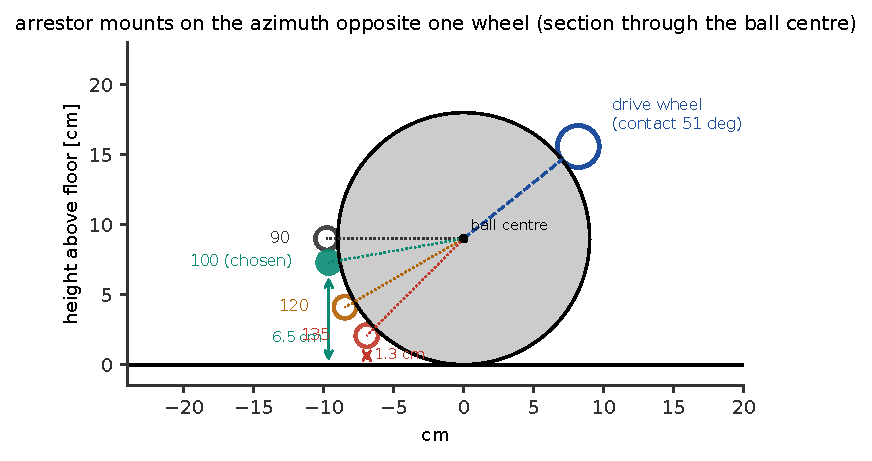
\includegraphics[width=0.9\columnwidth]{figures/study_retainer_geom.pdf}
\caption{Arrestor geometry: section through the ball centre on the azimuth opposite one wheel, mounts at 90, 100 (chosen), 120 and 135$^\circ$ with the upright floor clearance. Geometry only: no engine, randomisation, noise, worlds or seeds apply.}\label{fig:retgeom}
\end{figure}
\begin{table*}[t]\centering\footnotesize
\caption{Arrestor mount-angle sweep (zero-shot), corrected engine. Engine: Warp GPU (MuJoCo-Warp 3.17, float32), corrected for the S69 stale-subtree-mass error. Domain randomisation: on at scale 1. Observation noise: on. Worlds per cell: 1760 per cell (176 per terrain kind). Seeds: one policy (g12\_dr175\_s0, seed 0), trained without arrestors (zero-shot). Protocol: goal task of Table 2 with frictionless arrestors (radius 8 mm) added at evaluation; floor clearance from the geometry R + (R + r\_a) cos(phi) - r\_a; the floor-touch tilts marked with a dagger are from the study log (S79), and arrestor-floor contact is not simulated.}\label{tab:gen_sweep}
\resizebox{\textwidth}{!}{%
\begin{tabular}{lccccc}\toprule
Arrestor mount (polar angle from the top of the ball, deg) & Goal success undisturbed & Goal success pushes + pulls & Median misalignment at fall, undisturbed / disturbed [deg] & Arrestor bottom above the floor, upright [cm] & Tilt at which it touches the floor [deg]\\\midrule
none & 0.57 & 0.28 & 20.6 / 11.4 & n/a & n/a\\
135 (opposite the wheel) & 0.66 & 0.37 & 7.2 / 4.3 & 1.3 & 21$^\dagger$\\
120 & 0.69 & 0.39 & 5.4 / 3.2 & 3.3 & n/a\\
110 & 0.72 & 0.40 & 4.1 / 2.7 & 4.8 & n/a\\
100 & 0.75 & 0.45 & 3.4 / 1.8 & 6.5 & 57$^\dagger$\\
95 & 0.75 & 0.43 & 2.6 / 1.8 & 7.3 & n/a\\
90 (equator) & 0.76 & 0.44 & 2.7 / 1.7 & 8.2 & n/a\\
\bottomrule\end{tabular}}
\end{table*}

\begin{table}[t]\centering\footnotesize
\caption{Arrestor roller friction (zero-shot). Engine: Warp GPU (MuJoCo-Warp 3.17, float32), corrected for the S69 stale-subtree-mass error. Domain randomisation: on at scale 1. Observation noise: on. Worlds per cell: 1760 per cell. Seeds: one policy (g12\_dr175\_s0, seed 0), zero-shot. Protocol: goal task of Table 2, arrestors at 100 deg with the stated sliding friction (0 = ideal ball-transfer unit).}\label{tab:gen_friction}
\resizebox{\columnwidth}{!}{%
\begin{tabular}{lcc}\toprule
Arrestor sliding friction & Goal success undisturbed & Goal success pushes + pulls\\\midrule
0 & 0.75 & 0.45\\
0.05 & 0.74 & 0.42\\
0.2 & 0.76 & 0.42\\
\bottomrule\end{tabular}}
\end{table}


\paragraph{Results.} Added at evaluation to the policy trained without them, arrestors at 100$^\circ$ raise goal success by \gv{sw.gain_u} undisturbed and \gv{sw.gain_d} with pushes and pulls (Table~\ref{tab:gen_sweep}), the first change in this study that moves disturbance robustness; mounts between 90 and 100$^\circ$ are equal within noise, and 100$^\circ$ is chosen because only a mount below the equator resists lift-off. Trained with the arrestors (two seeds, Table~\ref{tab:gen_rettrain}, Fig.~\ref{fig:retainer}), the recipe improves every robustness measure at once: goal success \gv{fam.ret.u.1} undisturbed and \gv{fam.ret.d.1} with pushes and pulls against \gv{fam.dr175.u.1} and \gv{fam.dr175.d.1} without, and tile velocity falls \gv{fam.ret.velu} against \gv{fam.dr175.velu} undisturbed and \gv{fam.ret.veld} against \gv{fam.dr175.veld} disturbed; the gain grows with randomisation (\gv{fam.ret.u.2.5} against \gv{fam.dr175.u.2.5} at scale 2.5). Most of it is mechanical: zero-shot arrestors give about the same goal success at scale 1. \emph{Training with the arrestors costs tracking accuracy}: on the flat world the trained policies reach only \gv{ret.ach_min} to \gv{ret.ach_max} of the command against \gv{dr.ach_min} to \gv{dr.ach_max} without arrestors, on both seeds, while the arrestors themselves do not (\gv{zs.ach_min} to \gv{zs.ach_max} zero-shot). A second pure-learning seed confirms the first (\gv{pure.ach_min} to \gv{pure.ach_max} of the command, goal success \gv{goal.g12_pure_s1.u.success} undisturbed).
\begin{table*}[t]\centering\footnotesize
\caption{Training with the ball retainer, corrected engine. Engine: Warp GPU (MuJoCo-Warp 3.17, float32), corrected for the S69 stale-subtree-mass error. Domain randomisation: on (flat columns: off). Observation noise: on (flat columns: off). Worlds per cell: 1760 per goal and tile cell (176 per terrain kind); 64 per flat cell. Seeds: as listed (two seeds for the trained-with-retainer, ramped and pure rows). Protocol: eval\_battery.py; the retainer rows use the 100 deg arrestors in training and evaluation (RETAINER=0,0,0,100), the zero-shot row adds them only at evaluation; its flat row was not part of the S92 re-run, so its flat falls are measured on the old tile positions and overstated (error and achieved speed unaffected).}\label{tab:gen_rettrain}
\resizebox{\textwidth}{!}{%
\begin{tabular}{llccccc}\toprule
Policy & Arrestors & Goal success undisturbed, DR 1 / 1.75 / 2.5 & Goal success pushes + pulls, DR 1 / 1.75 / 2.5 & Tile velocity falls undisturbed / disturbed (DR 1) & Flat error at 0.3 / 0.6 / 0.9 [m/s] & Flat achieved / command\\\midrule
ramped recipe, seed 0 g12\_dr175\_s0 & none & 0.58 / 0.54 / 0.45 & 0.29 / 0.25 / 0.19 & 0.54 / 0.71 & 0.027 / 0.046 / 0.057 & 0.95 to 0.99\\
ramped recipe, seed 1 g12\_dr175\_s1 & none & 0.60 / 0.56 / 0.47 & 0.30 / 0.25 / 0.19 & 0.53 / 0.71 & 0.013 / 0.021 / 0.041 & 1.00 to 1.02\\
ramped recipe, seed 0 g12\_dr175\_s0 & added at evaluation (zero-shot) & 0.75 (scale 1 only) & 0.45 (scale 1 only) & 0.36 / 0.53 & 0.030 / 0.046 / 0.067 & 0.96 to 0.99\\
trained with the retainer, seed 0 g16\_ret100\_s0 & trained with & 0.71 / 0.70 / 0.62 & 0.46 / 0.42 / 0.35 & 0.31 / 0.49 & 0.049 / 0.140 / 0.188 & 0.81 to 0.86\\
trained with the retainer, seed 1 g16\_ret100\_s1 & trained with & 0.76 / 0.73 / 0.67 & 0.49 / 0.44 / 0.37 & 0.32 / 0.50 & 0.048 / 0.096 / 0.115 & 0.87 to 0.91\\
pure learning, seed 0 g12\_pure\_s0 & none & 0.44 / 0.43 / 0.37 & 0.26 / 0.23 / 0.18 & 0.32 / 0.54 & 0.130 / 0.260 / 0.406 & 0.55 to 0.60\\
pure learning, seed 1 g12\_pure\_s1 & none & 0.51 / 0.44 / 0.39 & 0.27 / 0.23 / 0.19 & 0.38 / 0.57 & 0.103 / 0.246 / 0.421 & 0.54 to 0.67\\
\bottomrule\end{tabular}}
\end{table*}


\paragraph{The authority trade-off and the recommended controller.} Pure learning trained with the arrestors (two seeds) is the most robust controller (goal success \gv{fam.pureret.u.1} undisturbed and \gv{fam.pureret.d.1} with pushes and pulls, tile velocity falls \gv{fam.pureret.velu} and \gv{fam.pureret.veld}) but tracks only \gv{fam.pureret.achmin} to \gv{fam.pureret.achmax} of the command; a tracking weight of 3 on the residual trained with arrestors does not recover tracking (\gv{fam.trk3.achmin} to \gv{fam.trk3.achmax}). With the arrestors the learned authority sets the trade-off (Table~\ref{tab:gen_tradeoff}, Fig.~\ref{fig:tradeoff}): above 0.25 tracking falls off while robustness rises and saturates, and below 0.25 robustness drops (\gv{fam.ret015.d.1} with pushes and pulls at 0.15) with no gain in tracking. We therefore recommend the LQR plus residual at authority 0.25 trained with the retainer (numbers in this paragraph are the g18 seeds at the training friction 0.001; the checkpoints retrained on the corrected contact model are in \S\ref{sec:retainer}, correction paragraph): achieved \gv{fam.ret025.achmin} to \gv{fam.ret025.achmax} of the command over three seeds (error at most \gvt{fam.ret025.errmax}\,m/s up to 0.9\,m/s), goal success \gv{goal.g18_ret_rs025_s0.u.success}, \gv{goal.g18_ret_rs025_s1.u.success} and \gv{goal.g18_ret_rs025_s2.u.success} undisturbed and \gv{goal.g18_ret_rs025_s0.d.success}, \gv{goal.g18_ret_rs025_s1.d.success} and \gv{goal.g18_ret_rs025_s2.d.success} with pushes and pulls (without arrestors \gv{fam.dr175.u.1} and \gv{fam.dr175.d.1}). Training it for 400M instead of 200M steps gives no gain (\gv{goal.g19_ret_rs025_400m_s0.u.success} and \gv{goal.g19_ret_rs025_400m_s0.d.success}). A single rendered clip shows a known weakness: at 0.6\,m/s up an 11$^\circ$ ramp it lags the command (0.40\,m/s at 2.8\,s) and falls at 5.6\,s. On held-out terrain (tile seed 1, Table~\ref{tab:gen_retheld}) the retainer gain holds (residual 0.5: \gv{rh.g16_ret100_s0.d} and \gv{rh.g16_ret100_s1.d} with pushes and pulls; pure learning \gv{rh.g16_pure_ret100_s0.d} and \gv{rh.g16_pure_ret100_s1.d}; without arrestors \gv{rh.g12_dr175_s0.d} and \gv{rh.g12_dr175_s1.d}).
On held-out terrain the recommended controller keeps its gain (\gv{rh.g18_ret_rs025_s0.u} and \gv{rh.g18_ret_rs025_s1.u} undisturbed, \gv{rh.g18_ret_rs025_s0.d} and \gv{rh.g18_ret_rs025_s1.d} with pushes and pulls). Its remaining falls are on discrete obstacles (Table~\ref{tab:gen_obstacles}): in the velocity task at 0.3\,m/s it falls on bumps in \gv{obs.bump} of worlds, large drops \gv{obs.large_drop}, step ups \gv{obs.step_up} and stairs \gv{obs.stairs}, but on flat tiles only \gv{obs.flat} and on ramps up \gv{obs.ramp_up}; a raw depth sensor does not reduce them. With 20\,s episodes, so that every robot reaches its feature, slowing the command from 0.3 to 0.1\,m/s did not reduce falls on the original contact model (\gv{spd.0.3.all} and \gv{spd.0.1.all} overall; Table~\ref{tab:gen_speedlong}), and a rule-based speed governor on the privileged height map barely helped (\gv{gov.none} to \gv{gov.oracle}); both readings were partly the standing blow-up described below and are corrected in the next paragraph. Feature size decides (Table~\ref{tab:gen_severity}, re-checked on the corrected model): step ups above about \gv{sev.step_up.split}\,cm fail in \gv{sev.step_up.large} of worlds against \gv{sev.step_up.small} below, and bumps above \gv{sev.bump.split}\,cm in \gv{sev.bump.large}; up-steps and bumps above about a quarter of the ball radius are nearly always fatal at any speed.
\paragraph{Correction: speed does matter on the corrected contact model.} Re-run at free-rolling friction 0.01 (Table~\ref{tab:gen_speed_mu01}), the speed test gives falls that rise monotonically with commanded speed, \gv{s100.spd.0.1.all} at 0.1\,m/s to \gv{s100.spd.0.9.all} at 0.9\,m/s; the old reading was inflated most at 0.1\,m/s (\gv{spd.0.1.all} against \gv{s100.spd.0.1.all}) because a creeping robot is nearly stationary, the blow-up condition. Size still dominates. The terrain-aware speed layer, dropped after the old measurement, was re-tested on a recommended checkpoint with 40\,s episodes so that a slowed robot still reaches its feature (Table~\ref{tab:gen_gov_mu01}): falls are \gv{sl40.none.all} with no layer, \gv{sl40.oracle.all} with a governor on the perfect height map and \gv{sl40.tof.all} with the head ToF sensor through a learned height estimator (precision 0.73, recall 0.85), both slowing to 0.05\,m/s near a discontinuity; the real effect is \gv{sl40.gain_min} to \gv{sl40.gain_max}, mostly on stairs (\gv{sl40.none.stairs} to \gv{sl40.oracle.stairs}) and bumps (\gv{sl40.none.bump} to \gv{sl40.oracle.bump}), at a cost of \gv{sl40.exitcost_min} to \gv{sl40.exitcost_max} in tile exits reached, and the goal task with 30\,s episodes agrees (\gv{sl30.none.fall} falls with no layer, \gv{sl30.tof05.fall} with the ToF layer). An earlier 15\,s version of this test appeared to halve obstacle falls; it was an exposure artefact, the slowed robots not having reached their feature. Obstacle falls are therefore set by obstacle size against ball size, and the tools that work are routing around what cannot be crossed (\S\ref{sec:nav}) and a larger ball (\S\ref{sec:scale}). A separate gap between the two checkpoint families, reported briefly in our log, was an evaluation bug, since fixed.
\begin{table*}[t]\centering\footnotesize
\caption{Falls against commanded speed on the corrected contact model (friction 0.01; 20\,s episodes). Engine: Warp GPU (MuJoCo-Warp 3.17, float32), corrected for the S69 stale-subtree-mass error; wheel-ball free-rolling friction 0.01 (S98), policy trained at 0.001. Domain randomisation: on at scale 1. Observation noise: on. Worlds per cell: 176 per terrain kind (1760 per row). Seeds: one policy (g18\_ret\_rs025\_s1, seed 1). Protocol: the Table 14 protocol: velocity task on the tiles, undisturbed, arrestors on, 20 s episodes so that every robot reaches its feature (eval\_governor.py with no governor; files speed\_mu01\_*.json); fall rate per kind; the last column repeats Table 14 at 0.001.}\label{tab:gen_speed_mu01}
\resizebox{\textwidth}{!}{%
\begin{tabular}{lccccccc}\toprule
Commanded speed & All tiles & step up & bump & large drop & stairs & flat & All tiles at 0.001 (Table 14, superseded)\\\midrule
0.1 m/s & 0.28 & 0.46 & 0.54 & 0.74 & 0.43 & 0.06 & 0.42\\
0.2 m/s & 0.34 & 0.61 & 0.73 & 0.72 & 0.48 & 0.05 & 0.41\\
0.3 m/s & 0.35 & 0.62 & 0.74 & 0.66 & 0.49 & 0.06 & 0.37\\
0.6 m/s & 0.40 & 0.54 & 0.66 & 0.77 & 0.51 & 0.11 & not run\\
0.9 m/s & 0.51 & 0.62 & 0.66 & 0.83 & 0.62 & 0.23 & not run\\
\bottomrule\end{tabular}}
\end{table*}

\begin{table*}[t]\centering\footnotesize
\caption{A terrain-aware speed layer with 40\,s episodes. Engine: Warp GPU (MuJoCo-Warp 3.17, float32), corrected for the S69 stale-subtree-mass error; wheel-ball free-rolling friction 0.01 (the policy's own training value, recorded in each file). Domain randomisation: on at scale 1. Observation noise: on. Worlds per cell: 176 per terrain kind (1760 per row). Seeds: one policy (g26\_ret\_rs025\_mu01\_s1, a recommended checkpoint), one evaluation seed. Protocol: velocity task at 0.3 m/s on the tiles, undisturbed, arrestors on, 40 s episodes so that a slowed robot still reaches its feature, tile seed 0; governor.py slow mode, which lowers the commanded speed to 0.05 m/s within 0.25 m of a rise above 2.4 cm or a drop above 8 cm, read from the perfect height map or from the ToF estimate; files gov\_vel03\_ps0\_{none,oracle\_v005,tof18\_v005}\_40s.json. An earlier 15 s version of this test (S100 to S102) let slowed robots run out of time before their feature and is superseded.}\label{tab:gen_gov_mu01}
\resizebox{\textwidth}{!}{%
\begin{tabular}{p{0.26\linewidth}cccccccc}\toprule
Speed layer (g26 seed 1) & Falls, all tiles & step up & bump & stairs & large drop & flat & Tile exit reached & Progress\\\midrule
no speed layer & 0.38 & 0.62 & 0.79 & 0.56 & 0.72 & 0.11 & 0.62 & 1.35 m\\
perfect height map, slow to 0.05 m/s near a discontinuity (upper bound) & 0.33 & 0.61 & 0.72 & 0.43 & 0.74 & 0.07 & 0.58 & 1.31 m\\
ToF sensor (18 x 14 zones) through a learned height estimator, slow to 0.05 m/s & 0.35 & 0.61 & 0.78 & 0.47 & 0.77 & 0.09 & 0.54 & 1.28 m\\
\bottomrule\end{tabular}}
\end{table*}

\begin{table*}[t]\centering\footnotesize
\caption{Tracking accuracy against robustness with the retainer, corrected engine. Engine: Warp GPU (MuJoCo-Warp 3.17, float32), corrected for the S69 stale-subtree-mass error. Domain randomisation: on (flat columns: off). Observation noise: on (flat columns: off). Worlds per cell: 1760 per goal and tile cell (176 per terrain kind); 64 per flat cell. Seeds: one per row as listed; authority 0.25 has three seeds (plus a 400M-step run), authority 0.5 and pure learning two. Protocol: eval\_battery.py; every row except the two references is trained and evaluated with the 100 deg arrestors; the zero-shot row adds them only at evaluation; its flat row was not part of the S92 re-run, so its flat falls are measured on the old tile positions and overstated (error and achieved speed unaffected).}\label{tab:gen_tradeoff}
\resizebox{\textwidth}{!}{%
\begin{tabular}{lcccccc}\toprule
Controller & Flat achieved / command (0.3 to 0.9 m/s) & Flat error at 0.9 m/s [m/s] & Goal success undisturbed, DR 1 / 1.75 / 2.5 & Goal success pushes + pulls, DR 1 / 1.75 / 2.5 & Tile velocity falls undisturbed / disturbed (DR 1) & Median goal time [s]\\\midrule
no arrestors (reference) g12\_dr175\_s0, seed 0 & 0.95 to 0.99 & 0.057 & 0.58 / 0.54 / 0.45 & 0.29 / 0.25 / 0.19 & 0.54 / 0.71 & 2.44\\
no arrestors (reference) g12\_dr175\_s1, seed 1 & 1.00 to 1.02 & 0.041 & 0.60 / 0.56 / 0.47 & 0.30 / 0.25 / 0.19 & 0.53 / 0.71 & 2.33\\
authority 0.5, arrestors added at evaluation only g12\_dr175\_s0, seed 0 & 0.96 to 0.99 & 0.067 & 0.75 (scale 1 only) & 0.45 (scale 1 only) & 0.36 / 0.53 & n/a\\
authority 0.15 g18\_ret\_rs015\_s0, seed 0 & 0.99 to 1.01 & 0.042 & 0.69 / 0.65 / 0.56 & 0.35 / 0.31 / 0.22 & 0.38 / 0.58 & 2.24\\
authority 0.25 (recommended) g18\_ret\_rs025\_s0, seed 0 & 0.99 to 1.01 & 0.036 & 0.71 / 0.68 / 0.60 & 0.42 / 0.36 / 0.29 & 0.34 / 0.55 & 2.44\\
authority 0.25 (recommended) g18\_ret\_rs025\_s1, seed 1 & 0.98 to 1.00 & 0.034 & 0.76 / 0.72 / 0.66 & 0.43 / 0.39 / 0.32 & 0.35 / 0.56 & 2.50\\
authority 0.25 (recommended) g18\_ret\_rs025\_s2, seed 2 & 0.90 to 0.99 & 0.049 & 0.76 / 0.71 / 0.63 & 0.44 / 0.41 / 0.32 & 0.36 / 0.55 & 2.68\\
authority 0.25, 400M steps g19\_ret\_rs025\_400m\_s0, seed 0 & 0.92 to 1.01 & 0.058 & 0.75 / 0.70 / 0.64 & 0.43 / 0.36 / 0.30 & 0.38 / 0.55 & 2.61\\
authority 0.35 g18\_ret\_rs035\_s0, seed 0 & 0.91 to 0.98 & 0.060 & 0.72 / 0.71 / 0.63 & 0.45 / 0.40 / 0.32 & 0.34 / 0.52 & 2.73\\
authority 0.5 g16\_ret100\_s0, seed 0 & 0.81 to 0.86 & 0.188 & 0.71 / 0.70 / 0.62 & 0.46 / 0.42 / 0.35 & 0.31 / 0.49 & 2.81\\
authority 0.5 g16\_ret100\_s1, seed 1 & 0.87 to 0.91 & 0.115 & 0.76 / 0.73 / 0.67 & 0.49 / 0.44 / 0.37 & 0.32 / 0.50 & 2.75\\
authority 0.5, tracking weight x3 g17\_ret100\_trk3\_s0, seed 0 & 0.74 to 0.88 & 0.201 & 0.71 / 0.68 / 0.62 & 0.49 / 0.43 / 0.36 & 0.32 / 0.46 & 3.10\\
soft LQR base, authority 0.5 g18\_ret\_soft\_s0, seed 0 & 0.69 to 0.76 & 0.266 & 0.75 / 0.75 / 0.66 & 0.51 / 0.47 / 0.39 & 0.29 / 0.49 & 2.96\\
pure learning (no LQR) g16\_pure\_ret100\_s0, seed 0 & 0.64 to 0.73 & 0.335 & 0.70 / 0.67 / 0.64 & 0.50 / 0.45 / 0.40 & 0.16 / 0.34 & 2.96\\
pure learning (no LQR) g16\_pure\_ret100\_s1, seed 1 & 0.65 to 0.82 & 0.325 & 0.74 / 0.73 / 0.67 & 0.50 / 0.46 / 0.40 & 0.19 / 0.38 & 2.62\\
\bottomrule\end{tabular}}
\end{table*}

\begin{table}[t]\centering\footnotesize
\caption{Where the recommended controller still falls (velocity task, undisturbed). Engine: Warp GPU (MuJoCo-Warp 3.17, float32), corrected for the S69 stale-subtree-mass error. Domain randomisation: on at scale 1. Observation noise: on. Worlds per cell: 176 per terrain kind. Seeds: as in the column headers. Protocol: velocity task at 0.3 m/s on the tiles, undisturbed (pushes and pulls off), 100 deg arrestors; fall rate per terrain kind, sorted by the seed-0 value.}\label{tab:gen_obstacles}
\resizebox{\columnwidth}{!}{%
\begin{tabular}{lccc}\toprule
Terrain kind & recommended, seed 0 (g18\_ret\_rs025\_s0) & recommended, seed 1 (g18\_ret\_rs025\_s1) & recommended + depth sensor, seed 0 (g20\_ret\_rs025\_depth\_s0)\\\midrule
flat & 0.08 & 0.07 & 0.08\\
ramp up & 0.12 & 0.14 & 0.11\\
step down & 0.16 & 0.16 & 0.19\\
rough & 0.17 & 0.16 & 0.23\\
small drop & 0.18 & 0.17 & 0.22\\
ramp down & 0.20 & 0.26 & 0.24\\
stairs & 0.48 & 0.52 & 0.51\\
step up & 0.61 & 0.62 & 0.55\\
large drop & 0.64 & 0.66 & 0.68\\
bump & 0.77 & 0.74 & 0.75\\
\bottomrule\end{tabular}}
\end{table}

\begin{table}[t]\centering\footnotesize
\caption{Falls against commanded speed (20\,s episodes). Engine: Warp GPU (MuJoCo-Warp 3.17, float32), corrected for the S69 stale-subtree-mass error. Domain randomisation: on at scale 1. Observation noise: on. Worlds per cell: 176 per terrain kind (1760 per row). Seeds: one policy (g18\_ret\_rs025\_s1, seed 1). Protocol: velocity task on the tiles, undisturbed, arrestors on, 20 s episodes so that every robot reaches the terrain feature (eval\_governor.py with no governor); fall rate per kind.}\label{tab:gen_speedlong}
\resizebox{\columnwidth}{!}{%
\begin{tabular}{lcccccc}\toprule
Commanded speed & All tiles & step up & bump & large drop & stairs & flat\\\midrule
0.1 m/s & 0.42 & 0.64 & 0.64 & 0.80 & 0.55 & 0.15\\
0.2 m/s & 0.41 & 0.66 & 0.80 & 0.73 & 0.56 & 0.08\\
0.3 m/s & 0.37 & 0.64 & 0.74 & 0.66 & 0.52 & 0.10\\
\bottomrule\end{tabular}}
\end{table}

\begin{table}[t]\centering\footnotesize
\caption{Falls against feature size (velocity task, 0.3\,m/s, 20\,s). Engine: Warp GPU (MuJoCo-Warp 3.17, float32), corrected for the S69 stale-subtree-mass error. Domain randomisation: on at scale 1. Observation noise: on. Worlds per cell: 352 per kind (two tile maps' worth of worlds, split into halves by severity). Seeds: one policy (g18\_ret\_rs025\_s1, seed 1). Protocol: velocity task at 0.3 m/s on the tiles, undisturbed, arrestors on, 20 s episodes; worlds split at the median drawn severity of their tile.}\label{tab:gen_severity}
\resizebox{\columnwidth}{!}{%
\begin{tabular}{lcccc}\toprule
Feature & Severity range on the map & Split & Falls, smaller half & Falls, larger half\\\midrule
step up & 1.1 to 5.9 cm & 2.3 cm & 0.40 & 0.95\\
bump & 1.4 to 3.6 cm & 2.4 cm & 0.59 & 0.90\\
stairs (riser) & 1.2 to 3.2 cm & 1.4 cm & 0.27 & 0.70\\
large drop & 10.9 to 18.3 cm & 15.1 cm & 0.61 & 0.77\\
small drop & 3.1 to 5.8 cm & 4.4 cm & 0.23 & 0.34\\
step down & 1.2 to 5.5 cm & 2.6 cm & 0.12 & 0.21\\
ramp up & 3.5 to 11.2 deg & 9.6 deg & 0.15 & 0.12\\
ramp down & 5.2 to 11.9 deg & 8.5 deg & 0.28 & 0.29\\
\bottomrule\end{tabular}}
\end{table}


\paragraph{A traction limit, not missing foresight.}\label{sec:traction} A driven ball of radius $r$ pressed against a step edge of height $h$ must lift off the floor and pivot on the edge; the contact normal makes an angle $\theta$ with the vertical, $\cos\theta=1-h/r$, and rolling over needs a tangential-to-normal force ratio $\tan\theta$, which friction supplies only if $\tan\theta<\mu$:
\begin{equation}
h<h_{\max}=r\big(1-\cos(\arctan\mu)\big),\qquad \mu\approx1:\ h_{\max}=r(1-\cos45^\circ)\approx0.29\,r,
\end{equation}
\gv{trac.h.0.09}\,cm for the 9\,cm ball and \gv{trac.h.0.135}\,cm for the 13.5\,cm ball (Fig.~\ref{fig:traction}); floor friction varies by surface class, so the limit varies per world. Run on the unseen 13.5\,cm-ball design, the recommended controller crosses up-steps and bumps the small ball cannot (Table~\ref{tab:gen_ballsize}: falls on the larger half of the step-up range \gv{bs.step_up.nom_l} to \gv{bs.step_up.big_l}, large bumps \gv{bs.bump.nom_l} to \gv{bs.bump.big_l}), while drops change little. A privileged height scan as policy input, the upper bound for any terrain sensor, does not reduce obstacle falls (Table~\ref{tab:gen_scan}). Pure learning falls less on large obstacles because it stalls in front of them and keeps balancing, not because it climbs (crossing \gv{stall.step_up.pc} on large step ups, against \gv{stall.step_up.lc} for the residual; Table~\ref{tab:gen_stall}). On this map the falls above the traction limit are therefore a physical limit of ball size and friction that foresight does not change; below it, slowing before a feature buys only \gv{sl40.gain_min} to \gv{sl40.gain_max} once the robot is given time to reach it (Table~\ref{tab:gen_gov_mu01}), and terrain sensing matters most for routing around obstacles, which these enclosed tiles do not allow (tested in \S\ref{sec:nav}).
\begin{table*}[t]\centering\footnotesize
\caption{Ball size against step height (traction-limit test). Engine: Warp GPU (MuJoCo-Warp 3.17, float32), corrected for the S69 stale-subtree-mass error. Domain randomisation: on at scale 1. Observation noise: on. Worlds per cell: 640 per terrain kind (64 per kind and design copy, two copies), split into halves by severity. Seeds: one policy (g18\_ret\_rs025\_s1, seed 1), trained on 9 cm-ball designs. Protocol: velocity task at 0.3 m/s on the tiles, undisturbed, arrestors on, 20 s episodes (eval\_governor.py with --eval-designs nom,nom against s1.5,s1.5).}\label{tab:gen_ballsize}
\resizebox{\textwidth}{!}{%
\begin{tabular}{lccc}\toprule
Feature & Smaller half / larger half of the severity range & Falls, nominal (9 cm ball): smaller / larger & Falls, s1.5 (13.5 cm ball, unseen design): smaller / larger\\\midrule
step up & 1.1 to 2.3 / 2.3 to 5.9 cm & 0.40 / 0.98 & 0.26 / 0.80\\
bump & 1.4 to 2.4 / 2.4 to 3.6 cm & 0.52 / 0.94 & 0.33 / 0.62\\
stairs (riser) & 1.2 to 1.4 / 1.4 to 3.2 cm & 0.17 / 0.67 & 0.19 / 0.64\\
large drop & 10.9 to 15.1 / 15.1 to 18.3 cm & 0.64 / 0.83 & 0.62 / 0.72\\
\bottomrule\end{tabular}}
\end{table*}

\begin{table*}[t]\centering\footnotesize
\caption{Privileged height scan as policy input against blind counterparts (retainer on). Engine: Warp GPU (MuJoCo-Warp 3.17, float32), corrected for the S69 stale-subtree-mass error. Domain randomisation: on at scale 1. Observation noise: on. Worlds per cell: 1760 per goal and tile cell, 176 per terrain kind. Seeds: one per row as listed (scan arms one seed each). Protocol: eval\_battery.py; the scan arms add the privileged 7 x 5 height scan ahead as a policy input (the upper bound for any terrain sensor); per-kind columns are falls in the 8 s velocity task at 0.3 m/s, undisturbed.}\label{tab:gen_scan}
\resizebox{\textwidth}{!}{%
\begin{tabular}{lcccccc}\toprule
Policy (all with the retainer) & Goal success undisturbed / disturbed (DR 1) & Tile velocity falls, undisturbed & step up falls & bump falls & stairs falls & large drop falls\\\midrule
residual 0.25 + scan g22\_ret\_rs025\_scan\_s0, seed 0 & 0.68 / 0.41 & 0.36 & 0.59 & 0.78 & 0.51 & 0.70\\
residual 0.25, blind g18\_ret\_rs025\_s0, seed 0 & 0.71 / 0.42 & 0.34 & 0.61 & 0.77 & 0.48 & 0.64\\
residual 0.5 + scan g22\_ret\_rs05\_scan\_s0, seed 0 & 0.74 / 0.53 & 0.32 & 0.55 & 0.71 & 0.45 & 0.63\\
residual 0.5, blind g16\_ret100\_s0, seed 0 & 0.71 / 0.46 & 0.31 & 0.53 & 0.56 & 0.42 & 0.68\\
residual 0.5, blind g16\_ret100\_s1, seed 1 & 0.76 / 0.49 & 0.32 & 0.54 & 0.65 & 0.43 & 0.68\\
pure learning + scan g22\_pure\_ret\_scan\_s0, seed 0 & 0.69 / 0.50 & 0.15 & 0.29 & 0.24 & 0.19 & 0.38\\
pure learning, blind g16\_pure\_ret100\_s0, seed 0 & 0.70 / 0.50 & 0.16 & 0.24 & 0.20 & 0.20 & 0.43\\
pure learning, blind g16\_pure\_ret100\_s1, seed 1 & 0.74 / 0.50 & 0.19 & 0.31 & 0.30 & 0.25 & 0.45\\
\bottomrule\end{tabular}}
\end{table*}

\begin{table}[t]\centering\footnotesize
\caption{Falls and crossings on the larger half of each obstacle range. Engine: Warp GPU (MuJoCo-Warp 3.17, float32), corrected for the S69 stale-subtree-mass error. Domain randomisation: on at scale 1. Observation noise: on. Worlds per cell: 640 per terrain kind, halved by severity. Seeds: one policy each (seed 1). Protocol: velocity task at 0.3 m/s on the tiles, undisturbed, arrestors on, 20 s episodes; crossed = left the tile upright past the feature.}\label{tab:gen_stall}
\resizebox{\columnwidth}{!}{%
\begin{tabular}{lcc}\toprule
Feature (larger half of the range) & Pure learning, retainer (g16\_pure\_ret100\_s1): falls / crossed & LQR + residual 0.25, retainer (g18\_ret\_rs025\_s1): falls / crossed\\\midrule
step up, larger half (2.3 to 5.9 cm) & 0.69 / 0.02 & 0.98 / 0.02\\
bump, larger half (2.4 to 3.6 cm) & 0.30 / 0.02 & 0.94 / 0.06\\
stairs (riser), larger half (1.4 to 3.2 cm) & 0.38 / 0.03 & 0.67 / 0.33\\
large drop, larger half (15.1 to 18.3 cm) & 0.58 / 0.39 & 0.83 / 0.17\\
\bottomrule\end{tabular}}
\end{table}

\begin{figure}[t]\centering
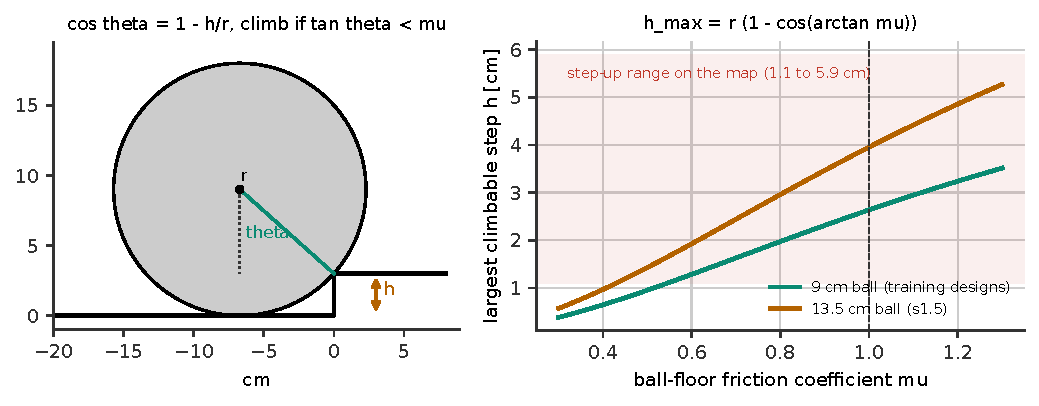
\includegraphics[width=\columnwidth]{figures/study_traction.pdf}
\caption{Traction limit for climbing a step: geometry (left, $r=9$\,cm, $h=3$\,cm) and the largest climbable step against friction for the two ball sizes (right), with the map's step-up range shaded. Analytical: no engine, randomisation, noise, worlds or seeds apply.}\label{fig:traction}
\end{figure}
\begin{table*}[t]\centering\footnotesize
\caption{The retainer on held-out terrain (tile seed 1), corrected engine. Engine: Warp GPU (MuJoCo-Warp 3.17, float32), corrected for the S69 stale-subtree-mass error. Domain randomisation: on at scale 1. Observation noise: on. Worlds per cell: 176 per terrain kind, 1760 per cell. Seeds: as listed. Protocol: goal task of Table 2 on a freshly generated tile map (tile seed 1); policies were trained on tile seed 0; the retainer rows run with the 100 deg arrestors.}\label{tab:gen_retheld}
\resizebox{\textwidth}{!}{%
\begin{tabular}{lcccc}\toprule
Policy & Undisturbed success, held-out map (tile seed 1) & trained map (tile seed 0) & Pushes + pulls success, held-out map & trained map\\\midrule
recommended: LQR + residual 0.25, trained with the retainer g18\_ret\_rs025\_s0, seed 0 & 0.66 & 0.71 & 0.38 & 0.42\\
recommended: LQR + residual 0.25, trained with the retainer g18\_ret\_rs025\_s1, seed 1 & 0.69 & 0.76 & 0.39 & 0.43\\
LQR + residual 0.5, trained with the retainer g16\_ret100\_s0, seed 0 & 0.66 & 0.71 & 0.42 & 0.46\\
LQR + residual 0.5, trained with the retainer g16\_ret100\_s1, seed 1 & 0.68 & 0.76 & 0.43 & 0.49\\
pure learning, trained with the retainer g16\_pure\_ret100\_s0, seed 0 & 0.66 & 0.70 & 0.46 & 0.50\\
pure learning, trained with the retainer g16\_pure\_ret100\_s1, seed 1 & 0.71 & 0.74 & 0.47 & 0.50\\
no arrestors (reference) g12\_dr175\_s0, seed 0 & 0.52 & 0.58 & 0.26 & 0.29\\
no arrestors (reference) g12\_dr175\_s1, seed 1 & 0.53 & 0.60 & 0.26 & 0.30\\
\bottomrule\end{tabular}}
\end{table*}

\begin{figure}[t]\centering
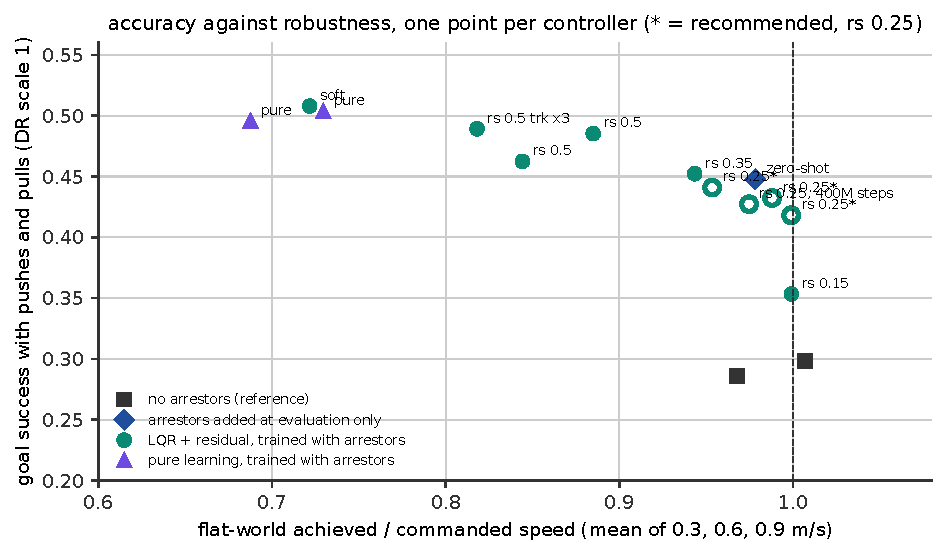
\includegraphics[width=\columnwidth]{figures/study_tradeoff.pdf}
\caption{Accuracy against robustness, one point per controller. Engine: Warp GPU, corrected. Randomisation: off on the horizontal axis (flat benchmark, 64 worlds per speed), on at scale 1 on the vertical axis (goal task with pushes and pulls, 1760 worlds). Noise: off (horizontal), on (vertical). Seeds: one point per seed. Protocol: Tables~\ref{tab:gen_flat} and~\ref{tab:gen_goal}; all points except the references use the 100$^\circ$ arrestors in training and evaluation.}\label{fig:tradeoff}
\end{figure}
\begin{figure*}[t]\centering
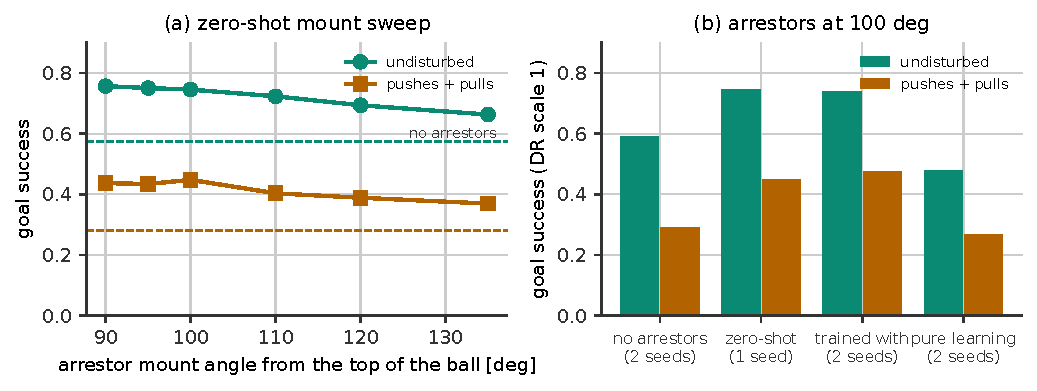
\includegraphics[width=0.85\textwidth]{figures/study_retainer.pdf}
\caption{The ball retainer. Engine: Warp GPU, corrected. Randomisation: on at scale 1. Noise: on. Worlds: 1760 per point or bar. Seeds: (a) one policy (g12\_dr175\_s0), zero-shot mount sweep, dashed lines without arrestors; (b) two seeds per bar except zero-shot (one). Protocol: goal task of Table~\ref{tab:gen_goal}.}\label{fig:retainer}
\end{figure*}

\paragraph{Correction: the 20\,s standing falls were a simulator blow-up.} Earlier drafts reported a 20\,s standing fall rate per design for the recommended controller, an LQR gain sweep on that test and a seed comparison; all are withdrawn. The wheel-ball contact pairs use anisotropic friction, 0.001 along the roller axis and 1.0 across it, and in the float32 engine that 1000 to 1 elliptic cone is ill-conditioned when the contact is nearly stationary: a standing robot at 1 to 2$^\circ$ of tilt can have its state turn non-finite in one 10\,ms step, preferentially where the ball is heavy relative to the body (kb4, bal025, zeta66). The termination rule counts a non-finite state as a fall, so these entered every 20\,s standing number (91\,\% of the standing ``falls'' of the worst seed were neither tips nor unseatings), while driving and the 8\,s battery were almost untouched. Contact buffers, solver, warm start, iteration counts, arrestors, randomisation and the height field were ruled out in a diagnostic of 880 standing worlds; raising the free-rolling coefficient to 0.01 removes the blow-up (0 of 880 non-finite against 0.127 at 0.001) with the real falls unchanged, and 0.01 is the model default from here (the coefficient of real rollers was never measured). Re-measured at 0.01 (Table~\ref{tab:gen_standing_mu01}; policies trained at 0.001), the recommended controller stands for 20\,s with \gv{mu.stand.all.min} and \gv{mu.stand.all.max} falls over 11 designs on two seeds, kb4 and bal025 at \gv{mu.stand.kb4.max} and \gv{mu.stand.bal025.max}, and drives at 0.3\,m/s with \gv{mu.drive.all.min} to \gv{mu.drive.all.max}. What remains is design specific and real: the quarter-mass ball unseats within the first second (\gv{mu.stand.kb025.min} to \gv{mu.stand.kb025.max} standing, \gv{mu.drive.kb025.min} to \gv{mu.drive.kb025.max} driving) and the four-times base mass falls in \gv{mu.drive.bal4.min} to \gv{mu.drive.bal4.max} of driving worlds. The earlier claim that the velocity integral is essential for standing is unverified. The recipe retrained at 0.01 (three seeds, g26\_ret\_rs025\_mu01) reproduces the picture: standing \gvt{mu.g26.stand.all.min} to \gvt{mu.g26.stand.all.max}, driving \gvt{mu.g26.drive.all.min} to \gvt{mu.g26.drive.all.max}, no non-finite world, so the two weak designs are properties of the recipe at these mass extremes. \emph{These three seeds replace the g18 seeds as the recommended checkpoints}; the recipe is unchanged and only the contact model is corrected, they are the only family with a reproducible standing number, and they equal the g18 seeds on a 15\,s obstacle course on the same contact model. Their standard battery: goal success \gv{g26.goal.1.u.min} to \gv{g26.goal.1.u.max} undisturbed and \gv{g26.goal.1.d.min} to \gv{g26.goal.1.d.max} with pushes and pulls at scale 1 (\gv{g26.goal.1.75.u.min} / \gv{g26.goal.1.75.d.min} to \gv{g26.goal.1.75.d.max} at 1.75, \gv{g26.goal.2.5.u.min} to \gv{g26.goal.2.5.u.max} / \gv{g26.goal.2.5.d.min} to \gv{g26.goal.2.5.d.max} at 2.5), tile velocity falls \gv{g26.vel.1.u.min} undisturbed and \gv{g26.vel.1.d.min} to \gv{g26.vel.1.d.max} disturbed, flat achieved \gv{g26.ach.0.3.min} to \gv{g26.ach.0.3.max} at 0.3\,m/s, \gv{g26.ach.0.6.min} to \gv{g26.ach.0.6.max} at 0.6 and \gv{g26.ach.0.9.min} to \gv{g26.ach.0.9.max} at 0.9 with no fall; every seed within 0.03 of the others (Tables~\ref{tab:gen_flat} and~\ref{tab:gen_goal}, rows ``corrected contact model''). The g18 seeds remain valid comparisons for every 8\,s result and for driving.
\begin{table*}[t]\centering\footnotesize
\caption{Standing and driving for 20\,s on flat interior tiles at wheel-ball free-rolling friction 0.01 (the earlier 20\,s standing tables are withdrawn, see text). Engine: Warp GPU (MuJoCo-Warp 3.17, float32), corrected for the S69 stale-subtree-mass error; wheel-ball free-rolling friction 0.01 for every row (the first two policies were trained at 0.001 and are evaluated at 0.01 through PAIR\_MU1; the retrained ones carry 0.01 in args.json; the value is recorded in each file's env\_settings). Domain randomisation: on at scale 1. Observation noise: on. Worlds per cell: 32 per design (352 per cell). Seeds: seeds 1 and 2 of the recommended recipe (seed 0 not re-measured) and the seeds of the recipe retrained at 0.01 that are evaluated so far, one evaluation seed each. Protocol: flat interior tiles (at least 7.5 m from the map border), 20 s episodes, arrestors on, no pushes or pulls; zero command (standing) or 0.3 m/s at a random heading (driving); no fall was at the map edge; a non-finite state is counted separately where the file records it (new evaluations only) and is 0.000 in every such row.}\label{tab:gen_standing_mu01}
\resizebox{\textwidth}{!}{%
\begin{tabular}{p{0.24\linewidth}ccc}\toprule
Policy & Standing still for 20 s at friction 0.01, falls: all 11 designs / kb025 / bal4 / kb4 / bal025 / zeta66 / nominal & Driving at 0.3 m/s for 20 s at 0.01, falls: all / kb025 / bal4 / kb4 / bal025 / zeta66 / nominal & Non-finite worlds (fraction)\\\midrule
recommended controller, seed 1 (trained at 0.001) g18\_ret\_rs025\_s1  & 0.03 / 0.24 / 0.05 / 0.00 / 0.00 / 0.00 / 0.00 & 0.06 / 0.50 / 0.18 / 0.00 / 0.00 / 0.00 / 0.00 & not recorded\\
recommended controller, seed 2 (trained at 0.001) g18\_ret\_rs025\_s2  & 0.04 / 0.29 / 0.13 / 0.00 / 0.00 / 0.00 / 0.00 & 0.07 / 0.54 / 0.23 / 0.00 / 0.00 / 0.00 / 0.02 & not recorded\\
same recipe retrained at 0.01, seed 0 g26\_ret\_rs025\_mu01\_s0  & 0.03 / 0.27 / 0.04 / 0.00 / 0.00 / 0.00 / 0.00 & 0.06 / 0.48 / 0.20 / 0.00 / 0.00 / 0.00 / 0.00 & 0.000\\
same recipe retrained at 0.01, seed 1 g26\_ret\_rs025\_mu01\_s1  & 0.03 / 0.28 / 0.06 / 0.00 / 0.00 / 0.00 / 0.00 & 0.07 / 0.53 / 0.22 / 0.00 / 0.00 / 0.00 / 0.00 & 0.000\\
same recipe retrained at 0.01, seed 2 g26\_ret\_rs025\_mu01\_s2  & 0.02 / 0.24 / 0.04 / 0.00 / 0.00 / 0.00 / 0.00 & 0.06 / 0.49 / 0.21 / 0.00 / 0.00 / 0.00 / 0.00 & 0.000\\
\bottomrule\end{tabular}}
\end{table*}


\subsection{Ball size against step size}\label{sec:scale}
The traction limit of \S\ref{sec:traction} predicts that the climbable step scales with the ball radius. To test it with one controller, the recommended recipe was trained (two seeds) on the 11 designs plus the robot scaled uniformly to 0.75, 1.5 and 2 times nominal (ball radius 6.75, 13.5 and 18\,cm; masses scaled with the cube of the size; Froude-scaled commands; arrestors re-fitted per size; its own planar model per size for the LQR), 14 designs in all, and evaluated at five sizes including a held-out 0.5 scale (4.5\,cm ball) on the same tile map with the same absolute feature sizes (Table~\ref{tab:gen_scale5}; cells are the mean of the two seeds, which agree within 0.1 on every large-feature cell). The four trained sizes are evaluated on the corrected contact model (wheel-ball free-rolling friction 0.01, see the correction above; policies trained at 0.001), the held-out 0.5 scale only at 0.001. Falls on up-steps and bumps fall monotonically with ball radius, in step with the limit: the taller step band (2.3 to 5.9\,cm) is fatal for the 6.75\,cm ball (\gv{sc.s0.75.step_up.l}), nearly fatal for 9\,cm (\gv{sc.nom.step_up.l}) and survivable for 13.5 and 18\,cm (\gv{sc.s1.5.step_up.l}, \gv{sc.s2.0.step_up.l}), whose limits (\gvo{sc.s1.5.hmax} and \gvo{sc.s2.0.hmax}\,cm) cover most of the band. Drops improve with size beyond what traction explains (larger drops \gv{sc.s0.75.large_drop.l} to \gv{sc.s2.0.large_drop.l}): in its own Froude time a bigger robot has longer to recover from a ledge that is a smaller fraction of its size. The held-out 4.5\,cm-ball robot fails almost everywhere, on flat ground too (\gv{sc.s0.5.flat}, at 0.001): the policy does not transfer that far down, and small ballbots are the hardest case. Against the first-pass evaluation at 0.001 the two small robots are unchanged (within \gv{sc.d_small_max} overall) because their falls are traction, while the two large robots lose \gv{sc.d_large_min} to \gv{sc.d_large_max} of overall falls and up to \gv{sc.d_step_max} at the large steps, where a stalled robot sits almost still at the riser (the blow-up condition); the size ordering and the design rule did not change. Binning the recorded height of every world's feature, both seeds pooled (Fig.~\ref{fig:ballsize}, Table~\ref{tab:gen_scalebins}) gives a fall curve per ball that rises from a floor of about 0.3 (the general 20\,s fall rate on terrain) to 1 and moves right with the radius. Its 50\,\% point sits at \gv{sc.p50r_min} to \gv{sc.p50r_max}\,$r$ across the four sizes and both features (mean \gv{sc.p50r_mean}\,$r$), below the nominal $0.29\,r$, because floor friction is randomised per world (0.4 to 1.2 by surface class; at $\mu=0.4$ the limit is only \gv{sc.mu_lo_frac}\,$r$), so the measured curve is the limit averaged over the friction distribution. The scale policy keeps the recommended controller's standard results on both seeds (Table~\ref{tab:gen_scalebatt}, scale seeds evaluated at friction 0.01 next to the recommended checkpoints: goal \gv{sc.batt.goal_u} to \gv{sc.batt.goal_u_max} undisturbed and \gv{sc.batt.goal_d} to \gv{sc.batt.goal_d_max} with pushes and pulls, flat achieved \gv{sc.batt.ach_min} to \gv{sc.batt.ach_max}). \emph{Design rule (simulation only):} choose a ball radius of about \gvo{sc.rule_lo} to \gvo{sc.rule_hi} times the tallest step to be climbed (from $0.29\,r$ at $\mu\approx1$ and from the mean measured 50\,\% point when friction is unknown), then add arrestors for the falls that are not traction.
\begin{table*}[t]\centering\footnotesize
\caption{Five robot sizes against the same obstacles (falls on the smaller / larger half of each feature range, mean of two training seeds; 0.5 scale one seed). Engine: Warp GPU (MuJoCo-Warp 3.17, float32), corrected for the S69 stale-subtree-mass error. Domain randomisation: on at scale 1 (floor friction 0.4 to 1.2 by surface class). Observation noise: on. Worlds per cell: 128 per terrain kind, robot scale and seed (1280 per scale and seed), split into halves at the midpoint of each feature's drawn range. Seeds: two training seeds of one recipe (g24\_scale\_rs025\_s0, g24\_scale\_rs025\_s1), the recommended recipe trained on the 11 designs plus the robot at 0.75, 1.5 and 2 times nominal size (14 designs); cells are the mean of the two seeds (the last column gives each seed); the 0.5 scale was never trained on and was evaluated with seed 0 only, at friction 0.001. Protocol: velocity task at 0.3 m/s Froude-scaled (times the square root of the scale) on the tiles, undisturbed, arrestors re-fitted per scale, 20 s episodes, tile seed 0; feature sizes are the same absolute sizes for every robot (eval\_governor.py --source none --eval-designs); evaluated at wheel-ball free-rolling friction 0.01 (S98) with policies trained at 0.001 (files stepsize\_mu01\_*.json).}\label{tab:gen_scale5}
\resizebox{\textwidth}{!}{%
\begin{tabular}{lccccccccc}\toprule
Robot scale & Ball radius & Predicted limit 0.29 r & Step up, falls: 1.1 to 2.3 / 2.3 to 5.9 cm & Bump: 1.4 to 2.4 / 2.4 to 3.6 cm & Stairs riser: below / above 1.4 cm & Large drop: 10.9 to 15.1 / 15.1 to 18.3 cm & Flat & All ten tile kinds & All ten tile kinds, per seed\\\midrule
0.5 (held out, not trained); at friction 0.001 only & 4.5 cm & 1.3 cm & 0.90 / 1.00 & 0.98 / 1.00 & 0.94 / 1.00 & 0.98 / 0.98 & 0.90 & 0.95 & 0.95 (seed 0 only)\\
0.75 & 6.75 cm & 2.0 cm & 0.49 / 1.00 & 0.77 / 0.99 & 0.34 / 0.82 & 0.84 / 0.89 & 0.13 & 0.46 & 0.46 | 0.46\\
1 (nominal) & 9 cm & 2.6 cm & 0.33 / 0.94 & 0.68 / 0.95 & 0.16 / 0.68 & 0.59 / 0.84 & 0.03 & 0.32 & 0.31 | 0.34\\
1.5 & 13.5 cm & 4.0 cm & 0.25 / 0.61 & 0.37 / 0.50 & 0.12 / 0.45 & 0.35 / 0.48 & 0.00 & 0.21 & 0.20 | 0.21\\
2 & 18 cm & 5.3 cm & 0.17 / 0.58 & 0.26 / 0.41 & 0.08 / 0.29 & 0.23 / 0.27 & 0.00 & 0.13 & 0.13 | 0.13\\
\bottomrule\end{tabular}}
\end{table*}

\begin{table*}[t]\centering\footnotesize
\caption{Falls against step and bump height in 1\,cm bins, by ball radius (both seeds pooled). Engine: Warp GPU (MuJoCo-Warp 3.17, float32), corrected for the S69 stale-subtree-mass error. Domain randomisation: on at scale 1 (floor friction 0.4 to 1.2). Observation noise: on. Worlds per cell: 36 to 128 per bin (the per-world feature heights of Table 30, binned, both seeds pooled). Seeds: 2 training seeds of the scale recipe (g24\_scale\_rs025\_s0, g24\_scale\_rs025\_s1). Protocol: as Table 30, evaluated at wheel-ball free-rolling friction 0.01 (S98); fall probability per 1 cm band of feature height.}\label{tab:gen_scalebins}
\resizebox{\textwidth}{!}{%
\begin{tabular}{lcccccccc}\toprule
Ball radius (predicted limit) & step up 1 to 2 cm & step up 2 to 3 cm & step up 3 to 4 cm & step up 4 to 5 cm & step up 5 to 6 cm & bump 1 to 2 cm & bump 2 to 3 cm & bump 3 to 4 cm\\\midrule
6.75 cm (limit 2.0 cm) & 0.36 & 0.86 & 1.00 & 1.00 & 1.00 & 0.57 & 0.87 & 0.99\\
9 cm (limit 2.6 cm) & 0.25 & 0.56 & 0.81 & 1.00 & 1.00 & 0.36 & 0.84 & 0.95\\
13.5 cm (limit 4.0 cm) & 0.21 & 0.36 & 0.33 & 0.72 & 0.76 & 0.33 & 0.38 & 0.50\\
18 cm (limit 5.3 cm) & 0.16 & 0.19 & 0.36 & 0.53 & 0.84 & 0.21 & 0.28 & 0.41\\
\bottomrule\end{tabular}}
\end{table*}

\begin{table*}[t]\centering\footnotesize
\caption{The scale policy on the standard battery at friction 0.01, against the recommended checkpoints. Engine: Warp GPU (MuJoCo-Warp 3.17, float32), corrected for the S69 stale-subtree-mass error; wheel-ball free-rolling friction 0.01 in every row (the scale seeds were trained at 0.001 and evaluated at 0.01 through PAIR\_MU1, files battery\_mu0.01.json; the recommended checkpoints were trained at 0.01). Domain randomisation: on at scale 1 for the goal columns (the 11 training designs of the goal task), off for the flat columns (nominal design). Observation noise: on (goal), off (flat). Worlds per cell: 1760 per goal cell, 64 per flat cell. Seeds: one row per training seed, as listed. Protocol: the standard battery (eval\_battery.py): goal task of Table 2 and the clean flat benchmark of Table 1 on interior tiles.}\label{tab:gen_scalebatt}
\resizebox{\textwidth}{!}{%
\begin{tabular}{p{0.3\linewidth}ccc}\toprule
Policy & Goal success, undisturbed / pushes and pulls (DR scale 1) & Flat benchmark, achieved over commanded speed at 0.3 / 0.6 / 0.9 m/s & Flat benchmark falls at 0.3 / 0.6 / 0.9 m/s\\\midrule
scale policy, 14 designs, trained at 0.001 g24\_scale\_rs025\_s0, seed 0, evaluated at 0.01  & 0.74 / 0.47 & 0.91 / 0.92 / 0.98 & 0.00 / 0.00 / 0.00\\
scale policy, 14 designs, trained at 0.001 g24\_scale\_rs025\_s1, seed 1, evaluated at 0.01  & 0.70 / 0.44 & 0.89 / 0.93 / 0.99 & 0.00 / 0.00 / 0.00\\
recommended checkpoint, 11 designs, trained and evaluated at 0.01 g26\_ret\_rs025\_mu01\_s0, seed 0  & 0.74 / 0.45 & 0.90 / 0.96 / 0.99 & 0.00 / 0.00 / 0.00\\
recommended checkpoint, 11 designs, trained and evaluated at 0.01 g26\_ret\_rs025\_mu01\_s1, seed 1  & 0.74 / 0.46 & 0.85 / 0.95 / 0.99 & 0.00 / 0.00 / 0.00\\
recommended checkpoint, 11 designs, trained and evaluated at 0.01 g26\_ret\_rs025\_mu01\_s2, seed 2  & 0.73 / 0.45 & 0.93 / 0.98 / 1.00 & 0.00 / 0.00 / 0.00\\
\bottomrule\end{tabular}}
\end{table*}

\begin{figure*}[t]\centering
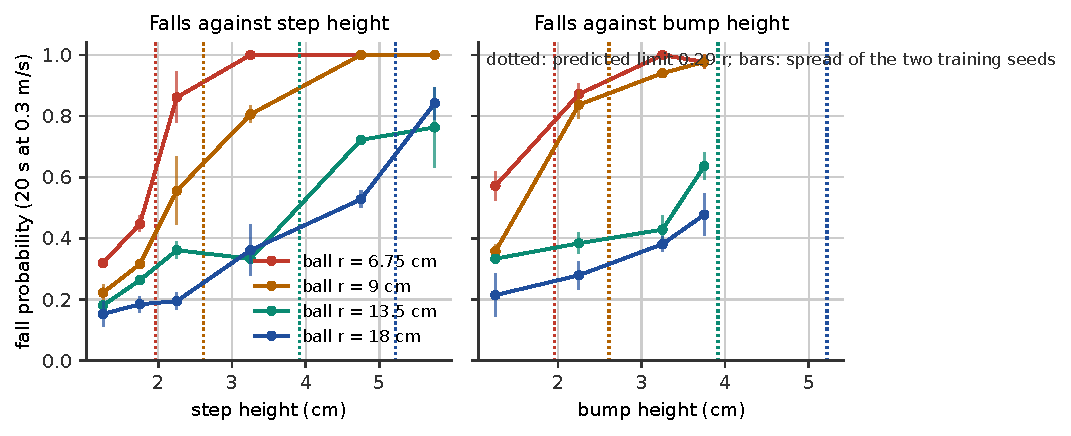
\includegraphics[width=0.9\textwidth]{figures/study_ballsize.pdf}
\caption{Fall probability against step height (left) and bump height (right) for four ball radii, 0.5\,cm bins with at least 8 worlds, worlds of both seeds pooled; vertical bars span the two seeds' values; dotted lines at the predicted limit $0.29\,r$; evaluated at wheel-ball free-rolling friction 0.01 (policies trained at 0.001). Engine: Warp GPU, corrected. Randomisation: on at scale 1 (floor friction 0.4 to 1.2). Noise: on. Worlds: 128 per terrain kind, size and seed, binned by drawn feature height. Seeds: two training seeds (g24\_scale\_rs025\_s0, s1). Protocol: velocity task at 0.3\,m/s Froude-scaled, undisturbed, arrestors on, 20\,s.}\label{fig:ballsize}
\end{figure*}

\subsection{Terrain-aware navigation and sensors}\label{sec:nav}
To test what terrain sensing does when obstacles can be avoided, every tile of a new map is a \emph{blocks} tile: flat ground with four 8\,cm blocks (three times the traction limit of the 9\,cm ball) across the tile axes 0.65 to 0.85\,m from the centre, 0.3 to 0.5\,m wide, plus up to two 24\,cm square blocks; the goal lies 1.2\,m away behind a block, and gaps between blocks are at least 0.7\,m. The balance controller is frozen; nothing is retrained. The results in this paragraph and the next were measured with the earlier checkpoint (g18, friction 0.001); the recommended checkpoint at its own friction is in Table~\ref{tab:gen_nav26}. A wavefront planner on top marks ground more than 3\,cm above the start as obstacle, inflates obstacles by the robot half-width plus margin (0.22\,m), computes a distance-to-goal field on a 64$\times$64 grid of 5\,cm cells every 0.2\,s, and steers toward the lowest-cost of 24 nearby points at up to 0.3\,m/s. With a sensor, each noisy range and the known sensor pose give a 3-D hit point; points more than 3\,cm above the ground under the ball are kept in a memory of the 600 most recent points that the planner rasterises. With the same controller (Table~\ref{tab:gen_nav}, Fig.~\ref{fig:nav}) the perfect height map cuts falls from \gv{nav.nav_blind.fall} to \gv{nav.nav_oracle.fall} and raises success from \gv{nav.nav_blind.success} to \gv{nav.nav_oracle.success}; a head-mounted ToF of 18$\times$14 zones reaches \gv{nav.nav_tof18_head.success}, a denser depth camera at the same mount \gv{nav.nav_cam32_head.success}. Mount and pitch matter more than resolution: pitched to $-40^\circ$ the camera leaves \gv{nav.nav_cam32_head_p40.stuck} of worlds stuck, an 8$\times$8 sensor or a low mount loses 7 to 12 points, and two body-cone sensors are worst (\gv{nav.nav_tof18_cones.success}). Under pushes and pulls even the perfect map falls \gv{nav.nav_oracle_pp.fall} (Table~\ref{tab:gen_navpp}); a wider margin (0.30 or 0.38\,m) closes the 0.7\,m gaps and leaves worlds stuck instead, so disturbance rejection near obstacles is the next limit.
\paragraph{Smooth motion to goals.} The wavefront planner picks a new neighbour every step, so its commanded heading jumps (RMS heading rate \gv{sm.o89.hr}\,rad/s). A smooth follower on the same distance field (carrot point 0.3\,m ahead, heading turned at most 2\,rad/s, speed lowered with heading error and changed at most 0.6\,m/s$^2$) cuts the rate to \gv{sm.oS.hr}\,rad/s for a few points of success (\gv{sm.oS.succ} against \gv{sm.o89.succ} with the perfect map; Table~\ref{tab:gen_smooth}); two faults found while tuning (a robot inside the inflated margin stopping for good, and a wider margin closing the 0.7\,m gaps) were fixed before any result was kept. With a real sensor the smooth follower first did worse (\gv{sm.navS_tof18.success}; \gv{sm.navS_tof18.over_block} of worlds rolled onto a block) because the gimbal yawed to the slowly turning command and saw side blocks late; aiming the sensor at the planner's target heading restores \gv{sm.navS_tof18_aim_w2.0.success} with block contacts \gv{sm.navS_tof18_aim_w2.0.over_block} (Table~\ref{tab:gen_smoothtof}); a proximity slow-down, faster turning and faster replanning were tried and rejected. \emph{Training with the planner in the loop} (30\,\% of training worlds on blocks tiles following the smooth planner, two seeds) is a null result: within seed noise of the frozen controller on every condition, with about \gv{nt.ob_gain_pp} fewer block contacts under pushes that do not turn into fewer falls (Table~\ref{tab:gen_navtrain}). The remaining failures are push recoveries near obstacles, a balance-controller limit, not a perception or training-data problem.
\paragraph{The recommended checkpoint on the corrected contact model.} Repeated with a recommended checkpoint (g26 seed 1) at friction 0.01 (Table~\ref{tab:gen_nav26}; smooth follower, sensor aimed at the target), ToF routing reaches \gv{nav26.tof.success} of goals behind a block, within \gv{nav26.tof_gap} of the perfect map (\gv{nav26.oracle.success}) and as smooth (heading-rate RMS \gv{nav26.tof.heading_rate_rms} against \gv{nav26.oracle.heading_rate_rms}\,rad/s); blind it reaches \gv{nav26.blind.success}. Under pushes and pulls about half the goals are reached (\gv{nav26.oracle_pp.success} with the perfect map, \gv{nav26.tof_pp.success} with the ToF), and a push near or onto a block remains the hard case.
\begin{table*}[t]\centering\footnotesize
\caption{Navigation with the recommended checkpoint at friction 0.01 (smooth follower). Engine: Warp GPU (MuJoCo-Warp 3.17, float32), corrected for the S69 stale-subtree-mass error; wheel-ball free-rolling friction 0.01, the controller's own training value. Domain randomisation: on at scale 1 (11 designs, floor classes). Observation noise: on (sensor ranges: noise 0.5 percent of range, 2 percent dropout). Worlds per cell: 528 per row (48 per design, 11 designs). Seeds: one controller seed (g26\_ret\_rs025\_mu01\_s1, a recommended checkpoint, frozen). Protocol: blocks map, 20 s, smooth follower (carrot 0.3 m, turn rate at most 2 rad/s; the blind row heads straight for the goal), sensor gimbal aimed at the planner's target heading; pushes 5 to 20 N and pulls 3 to 12 N in the last two rows; files g26\_ret\_rs025\_mu01\_s1/navS\_{blind,oracle,tof18}.json and navS\_{oracle,tof18}\_pp.json.}\label{tab:gen_nav26}
\resizebox{\textwidth}{!}{%
\begin{tabular}{lcccccc}\toprule
Hazard source (recommended checkpoint) & Reached goal & Fell & Stuck & Rolled onto a block & Median time to goal & Commanded heading-rate RMS [rad/s]\\\midrule
blind (straight to the goal) & 0.09 & 0.91 & 0.00 & 0.75 & 6.5 s & 2.21\\
perfect height map (upper bound) & 0.89 & 0.07 & 0.04 & 0.01 & 9.5 s & 1.69\\
ToF 18 x 14, head, pitched down 25 deg, aimed at the target heading & 0.84 & 0.07 & 0.08 & 0.04 & 10.8 s & 1.74\\
perfect height map, pushes and pulls & 0.57 & 0.39 & 0.04 & 0.16 & 8.6 s & 1.69\\
ToF 18 x 14, pushes and pulls & 0.51 & 0.43 & 0.06 & 0.17 & 9.4 s & 1.74\\
\bottomrule\end{tabular}}
\end{table*}

\begin{table*}[t]\centering\footnotesize
\caption{Navigation around unclimbable blocks (undisturbed), frozen recommended controller with a planner. Engine: Warp GPU (MuJoCo-Warp 3.17, float32), corrected for the S69 stale-subtree-mass error; earlier measurement: controller g18\_ret\_rs025\_s1 trained and evaluated at wheel-ball free-rolling friction 0.001 (the recommended checkpoint at 0.01 is in Table 37). Domain randomisation: on at scale 1 (11 designs, floor classes). Observation noise: on (sensor ranges: noise 0.5 percent of range, 2 percent dropout). Worlds per cell: 528 per row (48 per design, 11 designs). Seeds: one controller seed (g18\_ret\_rs025\_s1, frozen). Protocol: blocks map, undisturbed, 20 s episodes, goal 1.2 m away behind a block; wavefront planner (eval\_nav.py) with obstacles inflated by 0.22 m on a 5 cm grid; nothing is retrained.}\label{tab:gen_nav}
\resizebox{\textwidth}{!}{%
\begin{tabular}{lcccc}\toprule
Hazard source & Falls & Reached goal & Stuck & Rolled onto a block\\\midrule
blind (straight to the goal) & 0.91 & 0.09 & 0.00 & 0.74\\
privileged height map (upper bound) & 0.09 & 0.91 & 0.00 & 0.00\\
ToF 18 x 14, 55 x 42 deg, head, pitch -25 deg & 0.11 & 0.85 & 0.04 & 0.02\\
depth camera 32 x 24, 87 x 58 deg, head, pitch -25 deg & 0.12 & 0.83 & 0.05 & 0.02\\
depth camera 32 x 24, head, pitch -40 deg & 0.15 & 0.51 & 0.34 & 0.00\\
ToF 8 x 8, 45 x 45 deg, head, pitch -25 deg & 0.14 & 0.73 & 0.13 & 0.02\\
ToF 18 x 14 at the base origin, pitch -10 deg & 0.11 & 0.78 & 0.11 & 0.02\\
two ToF 18 x 14 on the body cones & 0.35 & 0.58 & 0.07 & 0.25\\
\bottomrule\end{tabular}}
\end{table*}

\begin{table*}[t]\centering\footnotesize
\caption{Navigation with pushes and pulls, and a wider planner margin. Engine: Warp GPU (MuJoCo-Warp 3.17, float32), corrected for the S69 stale-subtree-mass error; earlier measurement: controller g18\_ret\_rs025\_s1 trained and evaluated at wheel-ball free-rolling friction 0.001 (the recommended checkpoint at 0.01 is in Table 37). Domain randomisation: on at scale 1. Observation noise: on. Worlds per cell: 528 per row. Seeds: one controller seed (g18\_ret\_rs025\_s1, frozen). Protocol: as Table 19, with pushes 5 to 20 N and pulls 3 to 12 N (first three rows), and with the obstacle margin widened from 0.22 m to 0.30 or 0.38 m (last five rows; their disturbance setting is in the label).}\label{tab:gen_navpp}
\resizebox{\textwidth}{!}{%
\begin{tabular}{lcccc}\toprule
Hazard source & Falls & Reached goal & Stuck & Rolled onto a block\\\midrule
blind & 0.86 & 0.14 & 0.00 & 0.44\\
privileged height map & 0.41 & 0.58 & 0.01 & 0.13\\
ToF 18 x 14, head, pitch -25 deg & 0.52 & 0.45 & 0.03 & 0.15\\
ToF 18 x 14, margin 0.30 m (undisturbed) & 0.19 & 0.11 & 0.70 & 0.00\\
ToF 18 x 14, margin 0.38 m (undisturbed) & 0.28 & 0.00 & 0.71 & 0.00\\
ToF 18 x 14, margin 0.30 m, pushes + pulls & 0.62 & 0.14 & 0.24 & 0.17\\
ToF 18 x 14, margin 0.38 m, pushes + pulls & 0.62 & 0.01 & 0.38 & 0.21\\
privileged map, margin 0.38 m, pushes + pulls & 0.57 & 0.00 & 0.42 & 0.21\\
\bottomrule\end{tabular}}
\end{table*}

\begin{table*}[t]\centering\footnotesize
\caption{Smooth follower against the jerky wavefront planner (privileged map). Engine: Warp GPU (MuJoCo-Warp 3.17, float32), corrected for the S69 stale-subtree-mass error; earlier measurement: controller g18\_ret\_rs025\_s1 trained and evaluated at wheel-ball free-rolling friction 0.001 (the recommended checkpoint at 0.01 is in Table 37). Domain randomisation: on at scale 1. Observation noise: on. Worlds per cell: 528 per row (48 per design, 11 designs). Seeds: one controller seed (g18\_ret\_rs025\_s1, frozen). Protocol: blocks map, undisturbed, 20 s, privileged height map; the smooth follower (nav.py) tracks a carrot point 0.3 m down the same distance field, turns the commanded heading at most 2 rad/s, lowers speed with heading error and changes it at most 0.6 m/s$^2$. A dagger marks a value from the study log (the S89 file has no heading-rate field).}\label{tab:gen_smooth}
\resizebox{\textwidth}{!}{%
\begin{tabular}{lccccc}\toprule
Planner (privileged height map) & Reached goal & Falls & Stuck & Rolled onto a block & Commanded heading-rate RMS [rad/s]\\\midrule
S89 wavefront, best neighbour every step & 0.91 & 0.09 & 0.00 & 0.00 & 14.4$^\dagger$\\
smooth follower (carrot 0.3 m, turn rate at most 2 rad/s) & 0.86 & 0.14 & 0.00 & 0.04 & 1.7\\
\bottomrule\end{tabular}}
\end{table*}

\begin{table*}[t]\centering\footnotesize
\caption{Smooth following with the ToF sensor: variants. Engine: Warp GPU (MuJoCo-Warp 3.17, float32), corrected for the S69 stale-subtree-mass error; earlier measurement: controller g18\_ret\_rs025\_s1 trained and evaluated at wheel-ball free-rolling friction 0.001 (the recommended checkpoint at 0.01 is in Table 37). Domain randomisation: on at scale 1. Observation noise: on (sensor ranges noisy, with dropout). Worlds per cell: 528 per row. Seeds: one controller seed (g18\_ret\_rs025\_s1, frozen). Protocol: blocks map, undisturbed, 20 s; the head gimbal is yawed either to the command direction or to the planner's target heading (eval hook; on hardware the gimbal would be commanded by the navigation layer).}\label{tab:gen_smoothtof}
\resizebox{\textwidth}{!}{%
\begin{tabular}{lccccc}\toprule
Smooth follower with the ToF 18 x 14 sensor (head) & Reached goal & Falls & Stuck & Rolled onto a block & Commanded heading-rate RMS [rad/s]\\\midrule
smooth follower, sensor yawed along the command & 0.72 & 0.22 & 0.05 & 0.16 & 1.8\\
smooth follower, sensor aimed at the target heading, 2 rad/s (adopted) & 0.78 & 0.16 & 0.05 & 0.03 & 1.8\\
sensor aimed at the target heading, 4 rad/s & 0.76 & 0.17 & 0.07 & 0.04 & 3.3\\
rejected: faster turning, 4 rad/s, sensor along the command & 0.74 & 0.20 & 0.05 & 0.07 & 3.4\\
rejected: replanning every 0.04 s & 0.69 & 0.25 & 0.06 & 0.26 & 1.9\\
rejected: slow-down within 0.3 m of seen obstacles & 0.44 & 0.28 & 0.28 & 0.05 & 2.1\\
rejected: slow-down within 0.5 m & 0.26 & 0.29 & 0.46 & 0.03 & 2.2\\
S89 wavefront (jerky), for reference & 0.85 & 0.11 & 0.04 & 0.02 & 14.4$^\dagger$\\
\bottomrule\end{tabular}}
\end{table*}

\begin{table*}[t]\centering\footnotesize
\caption{Training with the planner in the loop against the frozen controller (null result). Engine: Warp GPU (MuJoCo-Warp 3.17, float32), corrected for the S69 stale-subtree-mass error; earlier measurement: controller g18\_ret\_rs025\_s1 trained and evaluated at wheel-ball free-rolling friction 0.001 (the recommended checkpoint at 0.01 is in Table 37). Domain randomisation: on at scale 1. Observation noise: on. Worlds per cell: 528 per cell. Seeds: one frozen controller seed against two planner-trained seeds. Protocol: blocks map, smooth follower (sensor along the command), 20 s; the planner-trained runs spent 30 percent of training worlds on blocks tiles following the smooth planner on the privileged map, otherwise the recommended recipe.}\label{tab:gen_navtrain}
\resizebox{\textwidth}{!}{%
\begin{tabular}{lccc}\toprule
Hazard source & frozen recommended controller (g18\_ret\_rs025\_s1): reached / fell / on block & planner-trained, seed 0 (g23\_nav\_rs025\_s0) & planner-trained, seed 1 (g23\_nav\_rs025\_s1)\\\midrule
perfect map, undisturbed & 0.86 / 0.14 / 0.04 & 0.85 / 0.13 / 0.01 & 0.85 / 0.14 / 0.02\\
perfect map, pushes + pulls & 0.55 / 0.44 / 0.20 & 0.55 / 0.43 / 0.13 & 0.57 / 0.42 / 0.13\\
ToF 18 x 14, undisturbed & 0.72 / 0.22 / 0.16 & 0.68 / 0.25 / 0.15 & 0.71 / 0.23 / 0.17\\
ToF 18 x 14, pushes + pulls & 0.41 / 0.56 / 0.22 & 0.43 / 0.53 / 0.18 & 0.46 / 0.51 / 0.21\\
\bottomrule\end{tabular}}
\end{table*}

\begin{figure}[t]\centering
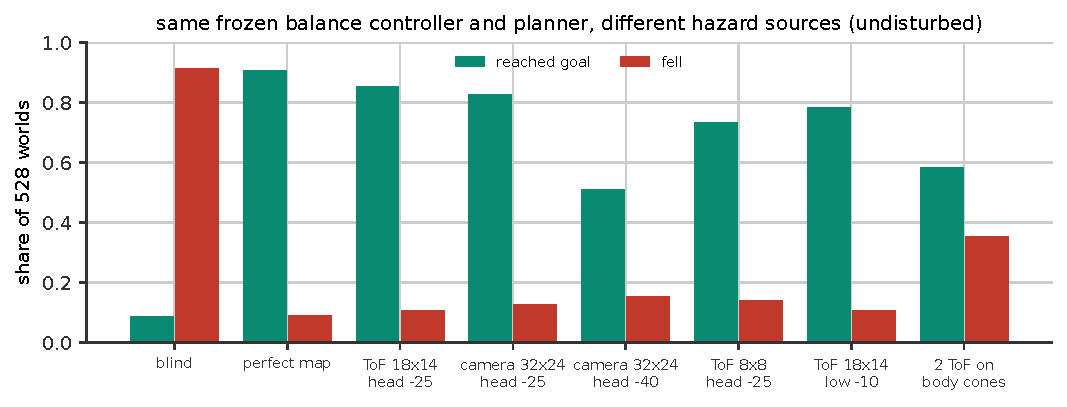
\includegraphics[width=\columnwidth]{figures/study_nav.pdf}
\caption{Navigation success and falls per hazard source. Engine: Warp GPU, corrected. Randomisation: on at scale 1. Noise: on (sensor ranges noisy, with dropout). Worlds: 528 per bar (48 per design, 11 designs). Seeds: one controller seed (g18\_ret\_rs025\_s1, frozen). Protocol: blocks map, undisturbed, 20\,s, wavefront planner with a 0.22\,m margin.}\label{fig:nav}
\end{figure}

\subsection{Smoother motion, adaptive authority and the current recommendation}\label{sec:motion}
\paragraph{Where the wobble came from.} The navigation paths above oscillate and robots sometimes hunt around a reached goal. In a recorded ToF run the planner's command turned smoothly (heading-rate RMS 1.6\,rad/s) while the ball's velocity heading swung at 8.1\,rad/s RMS and the robot made 66\,\% of the commanded speed: the oscillation lies in how the balance controller follows a continuously changing command, not in the planner. The policy had been trained on piecewise-constant commands, a ballbot must lean before it accelerates, and at the goal nothing held position. We therefore place a motion-reference layer between planner and controller (acceleration, braking and turn-rate limits, a braking profile $v=\sqrt{2ad}$ into the goal, and a position hold on arrival). Added to an unchanged policy it doubled the goal-test falls (0.15 to 0.31); trained with it (three seeds) it costs nothing on the battery and improves arrival and hold. Two further changes give the recommended recipe: \emph{adaptive authority} (0.15 while cruising, rising to 0.3 for about 0.5\,s when the command changes faster than 0.3\,m/s per second, nears zero, or the body tilts beyond $4^\circ$) and a \emph{goal dead band} (near the goal the higher authority stays on only while the ball moves faster than 0.05\,m/s).
\paragraph{The recommended controller and the variants that did not help.} Table~\ref{tab:gen_motion} compares every variant on a flat-tile goal test and on the standard battery. The recommended recipe (g34, three seeds) falls in \gv{mrf.g34.fall.min} to \gv{mrf.g34.fall.max} of goal tests against \gv{mr.g26_ret_rs025_mu01_s1.fall} for the previous checkpoint, holds at \gvt{mrf.g34.hold.min} to \gvt{mrf.g34.hold.max}\,m/s with \gv{mrf.g34.rev.min} to \gv{mrf.g34.rev.max} command reversals per world, and reaches \gv{mrf.g34.goal.1.u.min} to \gv{mrf.g34.goal.1.u.max} of battery goals undisturbed and \gv{mrf.g34.goal.1.d.min} to \gv{mrf.g34.goal.1.d.max} with pushes and pulls (g26: \gv{fam.ret025mu.u.min} to \gv{fam.ret025mu.u.max} and \gv{fam.ret025mu.d.min} to \gv{fam.ret025mu.d.max}). Four variants did not improve on it: a tracking reward weight of 3 (two seeds each on fixed and adaptive authority; curve tracking inside the seed spread); twice the training share for the three hard designs (three seeds; every battery cell within the spread, the hard designs still falling \gv{mrf.g35.hard.min} to \gv{mrf.g35.hard.max}); 400M instead of 200M steps (three seeds; fewer flat goal-test falls, \gvt{mrf.g36.fall.min} to \gvt{mrf.g36.fall.max}, but worse terrain goals in every battery cell and goal hunting back at \gv{mrf.g36.rev.min} to \gv{mrf.g36.rev.max} reversals per world); and training on 1.5 or 2 times stronger pushes and pulls (one seed each; pushed-battery success 0.02 to 0.04 lower). Three readings were corrected on the way: the goal hunting that motivated the dead band belonged to one seed, so the claim that adaptive authority \emph{needs} a dead band was withdrawn (the dead band is kept because it removes that seed-dependent behaviour at no cost); the zigzag falls of 0.28 to 0.33 measured terrain exposure, not turning (0.051 on a fully flat map); and solver constraint-buffer overflow warnings changed no battery cell by more than 0.02 when the buffers were quadrupled.
\begin{table*}[t]\centering\footnotesize
\caption{The motion-layer recipe and its variants (S110 to S116). Engine: Warp GPU (MuJoCo-Warp 3.17, float32), corrected for the S69 stale-subtree-mass error; wheel-ball free-rolling friction 0.01. Domain randomisation: on at scale 1 unless a column says 1.75 or 2.5 (training: ramped to 1.75). Observation noise: on. Worlds per cell: goal test 528 per row (48 per design, 11 designs); battery 1760 per cell (16 per design and terrain kind). Seeds: one per row; three seeds of the recommended recipe g34 (s0, s1, s2). Protocol: goal test: eval\_motion.py, goal 1.2 m away on flat interior tiles, 15 s, no pushes, commands through the motion layer for every run trained with it (the g26 row uses raw commands, as it was trained); hard designs = kb025 (light ball, 0.25 x ball mass), bal4 (heavy body, 4 x ballast) and tau6 (weak motors, 6 N m torque limit against 30). Battery: eval\_battery.py, goal task 1.1 m and velocity task 0.3 m/s on the tiled map, 8 s, surfaces on, arrestors on; pushes 5 to 20 N for 50 ms every 2 to 4 s and pulls 3 to 12 N for 0.5 to 2 s every 4 to 10 s. All recipes 200M steps except g36 (400M); files outputs/study/warp\_ppo/RUN/motion\_goal\_ref.json (g26: motion\_goal\_raw.json) and RUN/battery.json.}\label{tab:gen_motion}
\resizebox{\textwidth}{!}{%
\begin{tabular}{p{4.2cm}cccccccc}\toprule
Recipe (run) & Goal test: falls & Command reversals per world & Hold speed RMS [m/s] & Falls of the three hard designs (mean) & Battery goal success DR 1: undisturbed / pushes + pulls & DR 1.75 & DR 2.5 & Tile velocity falls DR 1: undisturbed / pushes + pulls\\\midrule
previous recommendation, raw commands, no motion layer (g26 s1) & 0.146 & 1.19 & 0.077 & 0.42 & 0.74 / 0.46 & 0.72 / 0.42 & 0.69 / 0.36 & 0.34 / 0.51\\
motion layer, fixed authority 0.25 (g29 s0) & 0.108 & 0.38 & 0.047 & 0.33 & 0.76 / 0.49 & 0.73 / 0.44 & 0.67 / 0.39 & 0.34 / 0.50\\
motion layer, fixed authority 0.25 (g29 s1) & 0.121 & 0.39 & 0.049 & 0.37 & 0.78 / 0.49 & 0.73 / 0.45 & 0.68 / 0.39 & 0.32 / 0.52\\
motion layer, fixed authority 0.25 (g29 s2) & 0.108 & 0.71 & 0.050 & 0.32 & 0.78 / 0.51 & 0.75 / 0.46 & 0.70 / 0.40 & 0.33 / 0.49\\
adaptive authority 0.15 / 0.3 (g32 s0) & 0.083 & 4.94 & 0.096 & 0.29 & 0.76 / 0.50 & 0.73 / 0.44 & 0.68 / 0.39 & 0.32 / 0.48\\
adaptive authority 0.15 / 0.3 (g32 s1) & 0.104 & 0.57 & 0.063 & 0.35 & 0.75 / 0.52 & 0.72 / 0.46 & 0.67 / 0.38 & 0.32 / 0.48\\
recommended: adaptive authority + goal dead band (g34 s0) & 0.104 & 0.67 & 0.058 & 0.32 & 0.79 / 0.51 & 0.77 / 0.47 & 0.69 / 0.39 & 0.32 / 0.48\\
recommended: adaptive authority + goal dead band (g34 s1) & 0.091 & 0.86 & 0.065 & 0.31 & 0.77 / 0.51 & 0.73 / 0.45 & 0.68 / 0.39 & 0.32 / 0.48\\
recommended: adaptive authority + goal dead band (g34 s2) & 0.110 & 0.48 & 0.052 & 0.30 & 0.78 / 0.52 & 0.75 / 0.45 & 0.69 / 0.39 & 0.31 / 0.48\\
adaptive + tracking reward 3 (g33 s0) & 0.100 & 0.99 & 0.068 & 0.33 & 0.77 / 0.53 & 0.75 / 0.45 & 0.70 / 0.41 & 0.32 / 0.48\\
adaptive + tracking reward 3 (g33 s1) & 0.081 & 1.38 & 0.060 & 0.29 & 0.77 / 0.51 & 0.73 / 0.45 & 0.67 / 0.38 & 0.30 / 0.48\\
adaptive + hard-design weighting (g35 s0) & 0.091 & 0.91 & 0.063 & 0.28 & 0.81 / 0.53 & 0.78 / 0.45 & 0.72 / 0.39 & 0.32 / 0.49\\
adaptive + hard-design weighting (g35 s1) & 0.108 & 0.40 & 0.059 & 0.29 & 0.79 / 0.52 & 0.77 / 0.45 & 0.72 / 0.39 & 0.31 / 0.49\\
adaptive + hard-design weighting (g35 s2) & 0.081 & 0.69 & 0.044 & 0.28 & 0.77 / 0.52 & 0.73 / 0.49 & 0.67 / 0.40 & 0.31 / 0.46\\
recommended + weighting, 400M steps (g36 s0) & 0.068 & 3.73 & 0.076 & 0.23 & 0.74 / 0.47 & 0.71 / 0.42 & 0.65 / 0.35 & 0.32 / 0.49\\
recommended + weighting, 400M steps (g36 s1) & 0.072 & 2.52 & 0.067 & 0.25 & 0.73 / 0.48 & 0.69 / 0.46 & 0.65 / 0.38 & 0.32 / 0.49\\
recommended + weighting, 400M steps (g36 s2) & 0.064 & 3.36 & 0.073 & 0.22 & 0.72 / 0.45 & 0.69 / 0.41 & 0.64 / 0.34 & 0.32 / 0.49\\
recommended, trained on 1.5 x pushes and pulls (g37 s0) & 0.136 & 1.58 & 0.082 & 0.37 & 0.79 / 0.49 & 0.76 / 0.43 & 0.70 / 0.36 & 0.34 / 0.50\\
recommended, trained on 2 x pushes and pulls (g37 s0) & 0.119 & 1.84 & 0.073 & 0.37 & 0.79 / 0.49 & 0.76 / 0.45 & 0.72 / 0.36 & 0.33 / 0.52\\
\bottomrule\end{tabular}}
\end{table*}

\paragraph{Navigation with the motion layer.} With the motion layer in the loop (Table~\ref{tab:gen_navmref}) ToF navigation reaches \gvt{nm.g34.tof18.success} of goals behind a block against \gvt{nm.g26.tof18.success} for the previous checkpoint, with the commanded heading-rate RMS cut from \gv{nm.g26.tof18.heading_rate_rms} to \gv{nm.g34.tof18.heading_rate_rms}\,rad/s, about a quarter. Running the same checkpoint with raw planner commands splits the gain: the success belongs to the checkpoint (\gvt{nm.g34raw.tof18.success} without the layer) and the whole wobble reduction to the layer (\gv{nm.g34raw.tof18.heading_rate_rms}\,rad/s without it). With a perfect map \gvt{nm.g34.oracle.success} arrive, so perception now limits ToF navigation; under pushes and pulls \gvt{nm.g34.tof18_pp.success}. The layer costs about \gvo{nm.layer_cost_s}\,s of median time per route; faster acceleration and braking limits were no better undisturbed and worse under pushes, and were rejected. One seed per recipe: success differences of 0.01 to 0.05 are within the seed spread, the wobble reduction is not. A contact escape layer for a robot with no terrain sensing (stall detection, obstacle memory, back up and re-plan; Table~\ref{tab:gen_escape}) reaches \gvt{esc.g34.bump_v15_40s.success} of goals on the new controller against \gvt{esc.g26.bump_v15_40s.success} on the previous one, with half as many robots stuck (\gv{esc.g34.bump_v15_40s.stuck} against \gv{esc.g26.bump_v15_40s.stuck}).
\begin{table*}[t]\centering\footnotesize
\caption{Navigation with the motion layer (S114). Engine: Warp GPU (MuJoCo-Warp 3.17, float32), corrected for the S69 stale-subtree-mass error; wheel-ball free-rolling friction 0.01. Domain randomisation: on at scale 1 (11 designs, floor classes). Observation noise: on (sensor ranges: noise 0.5 percent of range, 2 percent dropout). Worlds per cell: 528 (48 per design, 11 designs). Seeds: one controller seed per row, frozen. Protocol: eval\_nav.py on the blocks map (8 cm blocks, goal 1.2 m away behind a block), 20 s, smooth wavefront follower (carrot 0.3 m, turn limit 2 rad/s, v\_max 0.3 m/s), ToF on the head pitched down 25 deg and aimed at the planner target; for runs trained with the motion layer the planner command passes through motion\_ref.py (arrival braking, goal hold) unless NO\_MREF=1; pushes 5 to 20 N and pulls 3 to 12 N in the pushes column; files outputs/study/warp\_ppo/RUN/navS\_{tof18,tof18\_pp,oracle}[\_nomref].json.}\label{tab:gen_navmref}
\resizebox{\textwidth}{!}{%
\begin{tabular}{p{4cm}ccccccc}\toprule
Controller (motion layer in the loop or not) & ToF 18 x 14: reached / fell / stuck & Commanded heading-rate RMS [rad/s] & Command change per step & Median time to goal & ToF, pushes and pulls: reached / fell & Perfect map: reached / fell / stuck & Perfect map heading-rate RMS [rad/s]\\\midrule
previous recommendation, no motion layer (g26 s1; Table 37) & 0.845 / 0.072 / 0.083 & 1.74 & 0.50 & 10.8 s & 0.511 / 0.432 & 0.886 / 0.072 / 0.042 & 1.69\\
adaptive authority, with the motion layer (g32 s1) & 0.852 / 0.078 / 0.070 & 1.29 & 0.40 & 9.7 s & 0.544 / 0.400 & 0.926 / 0.064 / 0.009 & 1.23\\
recommended, with the motion layer (g34 s0) & 0.877 / 0.080 / 0.044 & 1.31 & 0.40 & 9.2 s & 0.557 / 0.413 & 0.938 / 0.061 / 0.002 & 1.23\\
recommended checkpoint, planner commands raw (g34 s0, NO\_MREF=1) & 0.881 / 0.070 / 0.049 & 1.79 & 0.51 & 8.9 s & not run & 0.915 / 0.083 / 0.002 & 1.74\\
\bottomrule\end{tabular}}
\end{table*}

\begin{table*}[t]\centering\footnotesize
\caption{Blind navigation with a contact escape layer (S109, S115). Engine: Warp GPU (MuJoCo-Warp 3.17, float32), corrected for the S69 stale-subtree-mass error; wheel-ball free-rolling friction 0.01. Domain randomisation: on at scale 1. Observation noise: on. Worlds per cell: 528 per row (48 per design, 11 designs). Seeds: one controller seed per pair of rows, frozen. Protocol: blocks map as Table 39 but no terrain sensing at all, 40 s episodes; escape layer experiments/warp\_ppo/escape.py through eval\_nav.py --source bump: stall detection (under 30 percent of the commanded speed for 1 s, no 0.1 m approach in 4 s, or tilt above 15 deg), a 0.3 m obstacle segment marked 0.2 m ahead, 1 s back-up at 0.15 m/s, re-plan, give up after 6 failures; files outputs/study/warp\_ppo/RUN/navS\_{blind,bump\_v15}\_40s.json.}\label{tab:gen_escape}
\resizebox{\textwidth}{!}{%
\begin{tabular}{p{5cm}ccccc}\toprule
Controller & Reached goal & Fell & Stuck & Rolled onto a block & Median time to goal\\\midrule
blind, straight at the goal previous recommendation g26 s1, no layer & 0.078 & 0.922 & 0.000 & 0.75 & 6.5 s\\
blind + contact escape (stall detection, obstacle memory, back up, re-plan), 0.15 m/s previous recommendation g26 s1, no layer & 0.547 & 0.237 & 0.216 & 0.55 & 14.7 s\\
blind, straight at the goal recommended g34 s0, motion layer & 0.017 & 0.983 & 0.000 & 0.81 & 6.0 s\\
blind + contact escape (stall detection, obstacle memory, back up, re-plan), 0.15 m/s recommended g34 s0, motion layer & 0.634 & 0.261 & 0.104 & 0.44 & 12.1 s\\
\bottomrule\end{tabular}}
\end{table*}

\paragraph{What the controller cannot absorb.} On a fully flat map (Table~\ref{tab:gen_limits}) the learned residual is what makes goal arrival work: \gv{lim.full.all} of robots fall with it, \gv{lim.lqr.all} with the LQR alone. The three hard designs are the light ball kb025 (0.25 times the ball mass), the heavy body bal4 (4 times the ballast) and the weak motors of tau6 (a 6\,N\,m torque limit against 30). The light ball is nearly impossible for the linear controller (\gv{lim.lqr.kb025}) and the residual saves part of it (\gv{lim.full.kb025}); the heavy body and the weak motors gain much less (\gv{lim.full.bal4} against \gv{lim.lqr.bal4}, \gv{lim.full.tau6} against \gv{lim.lqr.tau6}), which points to a design-space boundary rather than a training gap. Short pushes are absorbed fully (falls \gvt{lim.sw.push.all} against \gvt{lim.sw.none.all} undisturbed), sustained pulls up to about 3\,N as well (\gvt{lim.sw.p025.all}), and at the standard 3 to 12\,N \gv{lim.sw.p1.all} fall on flat ground; nearly all of the gap between undisturbed and pushed battery results is these sustained pulls. A steady pull needs a steady lean against an unseen force, which may need integral action that the LQR base lacks and an 80\,ms observation history cannot supply; this is being tested. All of this is simulation; there is no physical robot yet.
\begin{table*}[t]\centering\footnotesize
\caption{Limits on flat ground: hard designs and sustained pulls (S114, S116). Engine: Warp GPU (MuJoCo-Warp 3.17, float32), corrected for the S69 stale-subtree-mass error; wheel-ball free-rolling friction 0.01. Domain randomisation: on at scale 1. Observation noise: on. Worlds per cell: 528 per row in the first two rows (48 per design); 352 per row in the others (32 per design). Seeds: one controller seed (g34\_mref\_rsad\_db\_s0, recommended recipe), frozen. Protocol: TILES\_FLAT=1, so no terrain is involved. First two rows: eval\_motion.py goal test (1.2 m, 15 s, motion layer in the loop), files motion\_goal\_ref\_allflat[\_lqronly].json. Other rows: eval\_tiles2.py goal task (1.1 m, 8 s) with PUSH\_SCALE multiplying both the pushes and the sustained pulls, files eval2\_goal\_goal\_dr\_surf\_*\_flat\_noexit.json.}\label{tab:gen_limits}
\resizebox{\textwidth}{!}{%
\begin{tabular}{p{5.2cm}ccccc}\toprule
Test on a fully flat map (g34 s0) & Falls, all 11 designs & kb025 light ball (0.25 x ball mass) & bal4 heavy body (4 x ballast) & tau6 weak motors (6 N m) & the other eight designs\\\midrule
goal arrival, no disturbances: full controller (LQR + residual + motion layer) & 0.068 & 0.38 & 0.23 & 0.12 & at most 0.02\\
goal arrival, no disturbances: LQR alone (residual zeroed), same motion layer & 0.324 & 0.96 & 0.38 & 0.15 & 0.17 to 0.35\\
goal task 1.1 m, no pushes, no pulls & 0.074 & 0.42 & 0.17 & 0.13 & 0.00 to 0.07\\
goal task 1.1 m, short pushes only (5 to 20 N, 50 ms) & 0.078 & 0.40 & 0.19 & 0.13 & 0.00 to 0.08\\
goal task 1.1 m, pushes and pulls at 0.25 x (pulls 0.75 to 3 N) & 0.078 & 0.41 & 0.18 & 0.08 & 0.00 to 0.07\\
goal task 1.1 m, 0.5 x (pulls 1.5 to 6 N) & 0.139 & 0.47 & 0.18 & 0.11 & 0.01 to 0.58\\
goal task 1.1 m, 0.75 x (pulls 2.25 to 9 N) & 0.221 & 0.52 & 0.18 & 0.21 & 0.06 to 0.83\\
goal task 1.1 m, 1 x, the standard battery (pulls 3 to 12 N) & 0.361 & 0.59 & 0.18 & 0.47 & 0.17 to 0.93\\
\bottomrule\end{tabular}}
\end{table*}


\subsection{Generalisation to unseen robot designs}\label{sec:designs}
Two designs outside the 11 training designs were held out (Table~\ref{tab:gen_designs_ho}, Fig.~\ref{fig:designsho}): s1.5 (the robot scaled 1.5 times, ball radius 13.5\,cm, with its own planar model for the LQR base) and tau3 (a wheel torque limit of one tenth of nominal).\footnote{An earlier version of this evaluation computed the design vector relative to the first loaded design instead of the nominal one; it was fixed and re-run, and only the re-run is reported.} \emph{The LQR base carries a policy to an unseen robot}: the LQR-based controllers keep \gv{ho.lqr_min} to \gv{ho.lqr_max} on the larger robot, while pure learning with the retainer, the most robust controller on its training designs, collapses (\gv{ho.pure_min} to \gv{ho.pure_max}). The tenth-torque design is motor limited for every controller (at most \gv{ho.tau3_max}), and training on it does not help (\gv{ho.g21_ret_rs025_tau3_s0.u.tau3} and \gv{ho.g21_ret_rs025_tau3_s1.u.tau3}); training on 12 designs raises the unseen larger robot to \gv{ho.g21_ret_rs025_tau3_s0.u.s1.5} and \gv{ho.g21_ret_rs025_tau3_s1.u.s1.5} undisturbed (two seeds), with a seed-dependent gain under pushes and pulls.
\begin{table*}[t]\centering\footnotesize
\caption{Generalisation to unseen robot designs, corrected engine. Engine: Warp GPU (MuJoCo-Warp 3.17, float32), corrected for the S69 stale-subtree-mass error. Domain randomisation: on at scale 1. Observation noise: on. Worlds per cell: 160 per design (16 per terrain kind). Seeds: one per row as listed (two for the 12-design runs). Protocol: goal task of Table 2 on two designs outside the 11 training designs: s1.5 (robot scaled 1.5 times, ball radius 13.5 cm) and tau3 (wheel torque limit one tenth of nominal); the 12-design runs include tau3 in training, so for them only s1.5 is unseen.}\label{tab:gen_designs_ho}
\resizebox{\textwidth}{!}{%
\begin{tabular}{llcccc}\toprule
Policy & Trained on tau3 & Undisturbed: s1.5 (larger robot, unseen) & tau3 (one tenth torque) & Pushes + pulls: s1.5 & tau3\\\midrule
recommended: LQR + residual 0.25, retainer g18\_ret\_rs025\_s1, seed 1 & no & 0.71 & 0.30 & 0.66 & 0.15\\
LQR + residual 0.5, no retainer g12\_dr175\_s1, seed 1 & no & 0.69 & 0.15 & 0.61 & 0.12\\
pure learning, retainer g16\_pure\_ret100\_s1, seed 1 & no & 0.09 & 0.00 & 0.15 & 0.00\\
LQR + residual 0.25, retainer, 12 designs g21\_ret\_rs025\_tau3\_s0, seed 0 & yes & 0.89 & 0.29 & 0.76 & 0.17\\
LQR + residual 0.25, retainer, 12 designs g21\_ret\_rs025\_tau3\_s1, seed 1 & yes & 0.75 & 0.26 & 0.66 & 0.21\\
\bottomrule\end{tabular}}
\end{table*}

\begin{figure}[t]\centering
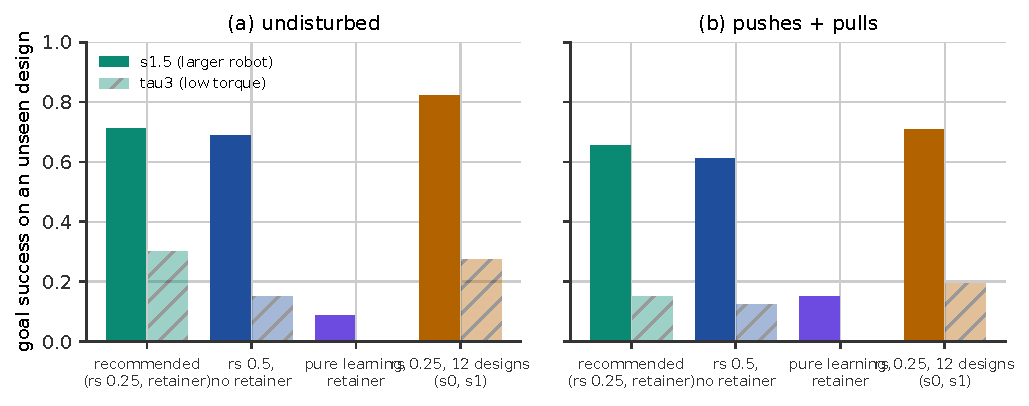
\includegraphics[width=\columnwidth]{figures/study_designs_ho.pdf}
\caption{Goal success on unseen robot designs. Engine: Warp GPU, corrected. Randomisation: on at scale 1. Noise: on. Worlds: 160 per bar (16 per terrain kind). Seeds: one per bar (seed 1); the 12-design bar averages two seeds. Protocol: goal task of Table~\ref{tab:gen_goal} on s1.5 (solid) and tau3 (hatched); tau3 is a training design for the 12-design runs.}\label{fig:designsho}
\end{figure}
\paragraph{Implications for a real robot (simulation only).} Four hypotheses follow for a hardware study, none tested on hardware: keep a model-based base controller with a small learned residual, since it transferred to a body unlike the training set while pure learning did not; add passive ball arrestors, which in simulation removed most falls without changing the controller's model; give the motors torque headroom, since with a tenth of the nominal torque every controller failed; and choose the ball radius for the steps that must be climbed, about \gvo{sc.rule_lo} to \gvo{sc.rule_hi} times the tallest step (\S\ref{sec:scale}).

\subsection{Perception}
The test is a controlled pair on the corrected engine: the ramped recipe with edge-focused starts, trained once with the 18$\times$14 head-mounted depth sensor (noisy, with dropout, learned end to end) and once blind, otherwise identically (200M steps, one seed each; Table~\ref{tab:gen_percarm}). \emph{The depth sensor gives no gain over the blind control}: goal success is \gv{goal.g15_edge_depth_s0.u.success} with depth against \gv{goal.g15_edge_blind_s0.u.success} blind undisturbed and \gv{goal.g15_edge_depth_s0.d.success} against \gv{goal.g15_edge_blind_s0.d.success} with pushes and pulls, the two differ by at most \gv{percarm.maxdiff} at any randomisation scale (about the seed and evaluation spread), and step up, stairs and bump are equal within noise; the tile velocity task falls slightly more with depth (\gv{vel.g15_edge_depth_s0.fall_u} against \gv{vel.g15_edge_blind_s0.fall_u}). \emph{Edge-focused starts alone do not move the baseline} (blind with edge starts \gv{goal.g15_edge_blind_s0.u.success} against \gv{goal.g12_dr175_s0.u.success} and \gv{goal.g12_dr175_s1.u.success} without). Each arm is a single seed, one sensor and an unchanged reward that does not value foresight; this shows that plain PPO did not learn to use this sensor, not that perception cannot help. A policy-shaped encoder pretrained to predict the height grid ahead reaches R$^2$ \gv{enc.depth_only_policy_shaped.R2} (Table~\ref{tab:gen_encoder}), weakest in the closest row because the $25^\circ$ downward pitch of the head mount leaves the nearest floor outside the zone grid; its frames came from a policy on the affected engine and no policy here uses it.
\begin{table*}[t]\centering\footnotesize
\caption{Depth sensor against blind control, both with edge-focused starts, corrected engine. Engine: Warp GPU (MuJoCo-Warp 3.17, float32), corrected for the S69 stale-subtree-mass error. Domain randomisation: on (flat error column: off). Observation noise: on (flat error column: off). Worlds per cell: 176 per terrain kind (1760 per cell); 64 for the flat column. Seeds: one seed per arm (seed 0), the reference rows are the two seeds of the ramped recipe. Protocol: goal task of Table 2 at DR scales 1, 1.75 and 2.5; the per-kind columns are undisturbed success at scale 1; tile velocity task at 0.3 m/s; both arms are the ramped recipe plus --edge-focus 0.5 and differ only by the depth sensor.}\label{tab:gen_percarm}
\resizebox{\textwidth}{!}{%
\begin{tabular}{lccccccccc}\toprule
Policy & Goal success DR 1: undisturbed / disturbed & DR 1.75 & DR 2.5 & Median time [s] & step up & stairs & bump & Tile velocity falls: undisturbed / disturbed & Flat error at 0.9 m/s\\\midrule
depth sensor (18x14, head mount) + edge starts g15\_edge\_depth\_s0, seed 0 & 0.60 / 0.29 & 0.53 / 0.26 & 0.45 / 0.18 & 2.36 & 0.36 & 0.44 & 0.27 & 0.56 / 0.73 & 0.044\\
blind control + edge starts g15\_edge\_blind\_s0, seed 0 & 0.60 / 0.28 & 0.54 / 0.23 & 0.47 / 0.19 & 2.30 & 0.38 & 0.41 & 0.28 & 0.53 / 0.73 & 0.046\\
reference: ramped recipe, no edge starts g12\_dr175\_s0, seed 0 & 0.58 / 0.29 & 0.54 / 0.25 & 0.45 / 0.19 & 2.44 & 0.31 & 0.44 & 0.26 & 0.54 / 0.71 & 0.057\\
reference: ramped recipe, no edge starts g12\_dr175\_s1, seed 1 & 0.60 / 0.30 & 0.56 / 0.25 & 0.47 / 0.19 & 2.33 & 0.39 & 0.47 & 0.20 & 0.53 / 0.71 & 0.041\\
\bottomrule\end{tabular}}
\end{table*}

The same sensor added on top of the recommended controller with the retainer (one seed, Table~\ref{tab:gen_percarm2}) also adds nothing: goal success \gv{goal.g20_ret_rs025_depth_s0.u.success} undisturbed and \gv{goal.g20_ret_rs025_depth_s0.d.success} with pushes and pulls, against \gv{fam.ret025.u.1} and \gv{fam.ret025.d.1} blind (three seeds), and obstacle falls unchanged within the seed spread.
\begin{table*}[t]\centering\footnotesize
\caption{Depth sensor on top of the recommended controller (retainer), corrected engine. Engine: Warp GPU (MuJoCo-Warp 3.17, float32), corrected for the S69 stale-subtree-mass error. Domain randomisation: on (flat column: off). Observation noise: on (flat column: off). Worlds per cell: 176 per terrain kind (1760 per goal or tile cell); 64 per flat cell. Seeds: one seed for the depth arm, three for the blind recommended controller. Protocol: eval\_battery.py with the 100 deg arrestors in training and evaluation; the depth arm also uses edge-focused starts.}\label{tab:gen_percarm2}
\resizebox{\textwidth}{!}{%
\begin{tabular}{lccccc}\toprule
Policy & Goal success undisturbed, DR 1 / 1.75 / 2.5 & Goal success pushes + pulls, DR 1 / 1.75 / 2.5 & Tile velocity falls undisturbed / disturbed (DR 1) & Step-up falls (velocity task) & Flat achieved / command\\\midrule
recommended + depth sensor (18x14) + edge starts g20\_ret\_rs025\_depth\_s0, seed 0 & 0.74 / 0.69 / 0.63 & 0.43 / 0.38 / 0.31 & 0.35 / 0.54 & 0.55 & 0.96 to 0.99\\
recommended, blind g18\_ret\_rs025\_s0, seed 0 & 0.71 / 0.68 / 0.60 & 0.42 / 0.36 / 0.29 & 0.34 / 0.55 & 0.61 & 0.99 to 1.01\\
recommended, blind g18\_ret\_rs025\_s1, seed 1 & 0.76 / 0.72 / 0.66 & 0.43 / 0.39 / 0.32 & 0.35 / 0.56 & 0.62 & 0.98 to 1.00\\
recommended, blind g18\_ret\_rs025\_s2, seed 2 & 0.76 / 0.71 / 0.63 & 0.44 / 0.41 / 0.32 & 0.36 / 0.55 & n/a & 0.90 to 0.99\\
\bottomrule\end{tabular}}
\end{table*}

\begin{table*}[t]\centering\footnotesize
\caption{Supervised depth-to-height encoder. Engine: Warp GPU (MuJoCo-Warp 3.17, float32). Domain randomisation: on in the data collection (see the caveat). Observation noise: on (depth zone noise 0.5 \% of range, 2 \% dropout). Worlds per cell: 606k frames from 2048 worlds, 11 designs; validation = 10 \% of worlds, split by world. Seeds: 1. Protocol: supervised regression of the height grid ahead and rise/drop hazards from an 18x14 simulated depth image; the driver policy is g2\_goal\_s0. Caveat: the frames were collected by a policy running on the engine before the S69 fix (stale subtree mass under mass randomisation). The metrics describe depth-to-height prediction, which does not depend on that artefact, but the frame distribution does.}\label{tab:gen_encoder}
\resizebox{\textwidth}{!}{%
\begin{tabular}{lccccc}\toprule
Encoder & R2 (7x5 height grid) & MAE [cm] & rise $\ge$ 2 cm F1 & drop $\ge$ 2 cm F1 & R2 by forward row (0.1 ... 1.3 m)\\\midrule
mean baseline & -0.00 & 3.87 & 0.00 & 0.00 & -0.00 -0.00 -0.00 -0.00 -0.00 -0.00 -0.00\\
proprio only & 0.02 & 3.97 & 0.25 & 0.20 & 0.04 0.05 0.04 0.02 -0.01 -0.02 -0.01\\
depth+proprio & 0.55 & 2.19 & 0.62 & 0.67 & 0.13 0.42 0.61 0.69 0.70 0.68 0.64\\
depth only policy shaped & 0.60 & 1.93 & 0.70 & 0.73 & 0.17 0.47 0.68 0.74 0.74 0.71 0.67\\
\bottomrule\end{tabular}}
\end{table*}

